\documentclass[twoside,a4paper]{report}
\usepackage[T1]{fontenc}
\usepackage[utf8]{inputenc}
\usepackage[english]{babel}
\usepackage{hyperref}
\usepackage[round]{natbib}
\usepackage{float}
\usepackage{ amssymb }
\usepackage{array, makecell}
\usepackage{booktabs, tabularx}
\newcolumntype{L}{>{\raggedright\arraybackslash}X}
\usepackage{setspace}
\usepackage{graphicx}
\usepackage{ amsmath}
\usepackage{csvsimple}
\usepackage{mathtools}
\usepackage{titling}
\usepackage{eqnarray}
\usepackage{endnotes}
\usepackage{lscape}
\usepackage{verbatim}
\usepackage{pdfpages}
\usepackage[toc,page]{appendix}
\usepackage{tikz}
\usetikzlibrary{shapes,arrows}
\usepackage[labelfont=bf]{caption}
\usepackage{subcaption}
\DeclareMathOperator*{\argmin}{arg\,min}
\DeclareMathOperator*{\argmax}{arg\,max}
\numberwithin{equation}{section} 
\renewcommand{\theequation}{Eq. \thesection.\arabic{equation}}
\newcolumntype{L}{>{\centering\arraybackslash}m{1.6cm}}
\newcolumntype{L}{>{\centering\arraybackslash}m{3cm}}
\usepackage[hmarginratio=1:1]{geometry}
\usetikzlibrary{calc}
\graphicspath{ {./images/} }
\newcommand{\subtitle}[1]{%
	\posttitle{%
		\par\end{center}
	\begin{center}\LARGE#1\end{center}
	\vskip0.5em}%
}




\begin{document}
%\maketitle

%%\textbf{ \Large ALBERT LUDWIGS UNIVERISTY OF FREIBURG}\\
%%
%%\vspace{0.5cm}
%
%%\Large MASTER THESIS
%%\Large{ALBERT LUDWIGS UNIVERISTY OF FREIBURG \\ MASTER THESIS}
%\vspace{0.5cm}
%
%
%\title{ \textbf{\Huge Multisite RNA-RNA Interaction Prediction} }	
%
%
%	
%\vspace{0.5cm}
%
%%\textbf{Author: \and Supervisor: }\smallskip{}
%%\\
%%Yogapriya Ayyanarmoorthy \and  Dr. Martin Raden \smallskip{}
%%\\
%
%%\author{Author:\\Yogapriya Ayyanarmoorthy \and Supervisor:\\ Dr. Martin Raden}
%
%
%
%%\large {A thesis submitted in fulfillment of the requirements for the degree of Master of Science in the Bioinformatics Group,	Department of Computer Science}
%%
%%\vspace{0.5cm}
%%
%% \large {Submitted on {\today}}  
 
 
 \begin{titlepage}
 	\begin{center}
 		
 		
 		{\scshape\Large ALBERT LUDWIGS UNIVERISTY OF FREIBURG \par}\vspace{0.8cm} % University name
 		\textsc{\Large MASTER THESIS} %\\[0.5cm] % Thesis type
 		
 		\vspace{0.5cm}
 		
 		\hrule  % Horizontal line
 			\vspace{0.4cm}
 		{\huge \bfseries  Multi-site RNA-RNA Interaction Prediction \par}
 		
 		\vspace{0.4cm} % Thesis title
 		\hrule  % Horizontal line
 		
 	\vspace{0.9cm}
 		
 		\begin{minipage}[t]{0.4\textwidth}
 			\begin{flushleft} \large
 				\emph{Author:}\\
 				\textit{Yogapriya Ayyanarmoorthy}  % Author name - remove the \href bracket to remove the link
 			\end{flushleft}
 		\end{minipage}
 		\begin{minipage}[t]{0.4\textwidth}
 			\begin{flushright} \large
 				\emph{Supervisor:} \\
 				\textit{Dr. Martin Raden}
 				%\href{http://www.jamessmith.com}{} % Supervisor name - remove the \href bracket to remove the link  
 			\end{flushright}
 		\end{minipage}\\[1cm]
 	\begin{minipage}[t]{0.4\textwidth}
 		\begin{center} \large
 			\emph{Examiner:} \\
 			\textit{Prof.~Dr. Rolf Backofen (Bioinformatics, University of Freiburg)}\\
 			\textit{Prof. Dr. Sebastian A. Will (AMIBio, Laboratoire d'informatique de l'École Polytechnique, IPP, France)}
 			%\href{http://www.jamessmith.com}{} % Supervisor name - remove the \href bracket to remove the link  
 		\end{center}
 	\end{minipage}%\\[3cm]
 	
 		
 	\vspace{1.5cm}
 		
 		\large {A thesis submitted in fulfillment of the requirements\\ for the degree of Master of Science\\
 		in the Bioinformatics Group,\\	Department of Computer Science} %[0.4cm]
 	
 	\vspace{0.9cm}
 		
 		{\large {Submitted on \today}}%\\[4cm] % Date
 		%\includegraphics{Logo} % University/department logo - uncomment to place it
 		
 		\vfill
 		
 	\end{center}
 \end{titlepage}
 
\pagenumbering{roman}
\newpage
%\chapter*{DECLARATION}
\begin{center}

\textbf{ \Large DECLARATION}\\
	
\end{center}
 	\vspace{0.9cm}
I hereby declare, that I am the sole author and composer of my Thesis and that no
other sources or learning aids, other than those listed, have been used. Furthermore, I declare that I have acknowledged the work of others by providing detailed references of said work. I hereby also declare, that my Thesis has not been prepared for another examination or assignment, either wholly or excerpts thereof.
\\

\hfill%
\vspace{0.9cm}

\begin{tabular}[t]{c}
	
	\rule{10em}{0.4pt}\\ Place , Date
\end{tabular}%
\hfill%
\begin{tabular}[t]{c}
	\rule{10em}{0.4pt}\\ Signature
\end{tabular}%


\newpage

I would like to thank Prof. Dr. Rolf Backofen so much for offering me this great opportunity to work on my Master Thesis in his group of Bioinformatics in Albert Ludwigs University of Freiburg.\\

I owe a lot to my supervisor Dr. Martin Raden, this thesis would not have been possible without his continuous guidance and support with both knowledge and ideas throughout the research. I want to thank him a lot for all his efforts, for providing me with thorough feedback and help throughout my work. Working with him was a great pleasure for me.\\

I am also grateful to my respectful parents for their great support along my stay,
without whom I wouldn’t have been able to stay abroad.\\

I want to thank my friends for being helpful and friendly, which contributed positively to my work.
 \\


\newpage
\chapter*{Abstract}
\addcontentsline{toc}{chapter}{Abstract}
%Abstract in English

Ribonucleic acid (RNA) is an essential biological macromolecule in all biological cells. Computational prediction techniques may be used to determine how two RNA molecules will form intermolecular base pairing. A variety of biophysical and biochemical approaches are there to test the RNA-RNA interactions (RRIs). At very large computational expense, there are a range of algorithms in the literature that can anticipate a lot of these interactions.\\

 The identification of non-coding (nc)RNA targets is largely regulated by two factors, namely the consistency of the duplex between the two interacting RNAs and the internal structure of both mRNA and ncRNA. Approaches may also be divided between various major categories based on whether they consider the inter- and intramolecular structure. One such approach is accessibility based interaction prediction model, which helps us in finding the single-site interaction of two RNAs. IntaRNA is a tool for rapid and precise prediction of interactions for accessibility based approach.  \\

 Within this thesis, we developed a model using iterative scheme which predicts concurrent blocks of interactions within an accessibility based prediction model and provides us with the prediction of  joint structure for the interacting RNAs and total energy. The proof for the energy of an respective Multi-site RRI are computed from the two energies is also shown. The respective extensions of the IntaRNA package will be included in the main package for external usage and further development. The comparison between various RNAs molecules have been tested and the output is been provided with polygon plots. Further to that, alternative RRIs prediction approaches and advance improvements and drawbacks are discussed within the thesis. \\



\newpage
\chapter*{Zusammenfassung}
\addcontentsline{toc}{chapter}{Kurzfassung} 
%Kurzfassung auf Deutsch

Ribonukleinsäure (RNA) ist ein essentielles biologisches Makromolekül in allen biologischen Zellen. Computergestützte Vorhersagetechniken können verwendet werden, um zu bestimmen, wie zwei RNA-Moleküle eine intermolekulare Basenpaarung bilden. Es gibt verschiedene biophysikalische und biochemische Ansätze, um die RNA-RNA-Wechselwirkungen (RRIs) zu testen. Bei sehr hohem Rechenaufwand gibt es in der Literatur eine Reihe von Algorithmen, die viele dieser Wechselwirkungen antizipieren können. \\

Die Identifizierung von durch nicht-kodierende RNAs regulierten RNAs wird weitgehend durch zwei beeinflusst reguliert, nämlich die Konsistenz des Duplex zwischen den beiden interagierenden RNAs und die interne Struktur von mRNA und ncRNA. Ansätze können auch in verschiedene Hauptkategorien unterteilt werden, je nachdem, ob sie das inter- und intramolekulare Gerüst berücksichtigen. Ein solcher Ansatz ist das auf Accessibility basierende Interaktionsvorhersagemodell, das uns hilft, die Single-Site-Interaktion zweier RNAs zu finden. IntaRNA ist ein Werkzeug zur schnellen und präzisen Vorhersage von Interaktionen für mit Hilfe eines solchen Accessibility basierenden Ansatz.  \\

In dieser Arbeit haben wir ein Modell entwickelt, das gleichzeitig auftretende Interaktionen mit Hilfe eines auf Accessibility basierenden modells vorhersagt. Der Beweis für die Energie eines jeweiligen RRI mit mehreren Standorten, der aus den beiden Energien berechnet wird, wird ebenfalls gezeigt. Die jeweiligen Erweiterungen des IntaRNA-Pakets werden zur externen Verwendung und Weiterentwicklung in das Hauptpaket aufgenommen. Der Vergleich zwischen verschiedenen RNAs-Molekülen wurde getestet und mit Polygon-Plots visualisiert. Darüber hinaus diskutierten wir über den Vergleich zwischen den RRI-Vorhersageansätzen und über Verbesserungen und Nachteile.\\


	
%	\maketitle
	
	\tableofcontents
	 	
	\chapter{Introduction}
	\pagenumbering{arabic}
	RNA molecules play important roles in various biological processes. Their regulation and function are mediated by interacting with other molecules, e.g by forming base pairs between two RNAs, called RNA-RNA interactions (RRI).  Many RNAs interact via multiple synchronous, non-overlapping subinteractions (M-RRI), e.g. OxyS-fhlA. There are fast and reliable single interaction site (S-RRI) prediction tools like IntaRNA, which helps us in predicting mRNA target sites for given non-coding RNAs (ncRNAs) , also they are capable of modelling all sites individually but not in a joint prediction. The simultaneous prediction of both intra- and inter-molecular base pairing allowing for multiple sites is computationally expensive. Some known approaches are IRIS, piRNA, NUPACK. Here we use a S-RRI prediction tool (namely IntaRNA) for the prediction of M-RRI.
	
	\section{Biological Background of RNA}
	In this thesis, I will focus on Ribonucleic acids (RNA). First of all, I would like to provide the basic biological background that is essential for the thesis. Ribonucleic acid, or RNA is one of the three major biological macromolecules that are important for all known forms of life (along with DNA (deoxyribonucleic acid) and proteins). The interaction between two RNAs plays a vital role in the basic cellular activities like transcription, RNA processing and translation. The process by which DNA is copied to RNA is called \textit{transcription}, and that by which RNA is used to produce proteins is called \textit{translation}. RNAs also play an important role in protein synthesis. \\
	
	 DNA is double stranded and RNA is a single-stranded molecule. Each strand of RNA is a sequence of four building blocks called \textit{nucleotides}. Each nucleotide contains sugar, phosphate and nitrogen containing bases. The sugar and phosphate groups form the backbone of RNA strand and the bases bond to each other. The RNA molecules are represented as a sequence $S \in \{A, C, G, U\} ^*$, where A (adenine), C (cytosine), G (guanine), U (uracil) are the bases of the nucleotide chain.\\
	 
	According to their potential for coding, RNA's are classified into two major categories i.e., coding RNAs and noncoding RNAs. Coding RNAs mostly refers to mRNA that encodes protein to act as different components including cell structures, signal transductors and enzymes. Noncoding RNAs act as cellular regulators with no protein encoding.\\
	Complementary bases $C$-$G$ and $A$-$U$ form stable base pairs with each other using hydrogen bonds. These are called Watson-Crick pairs. Also important are the weaker $U$-$G$ wobble pairs. Together they are called \textit{canonical base pairs}. In general, isolated base pairs are unstable. If interacting bases belong to the same molecule of RNA, they form \textit{intra-molecular} structures and if they belong to different molecules of RNA, they form \textit{inter-molecular} structures.\\
	
	The prediction of RNA-RNA interaction is intended to predict these intermolecular structures between two RNA molecules, an extremely important step in understanding the role of ncRNAs. However, intramolecular and intermolecular structures are not mutually exclusive.\\
	
	\begin{figure}[h]
	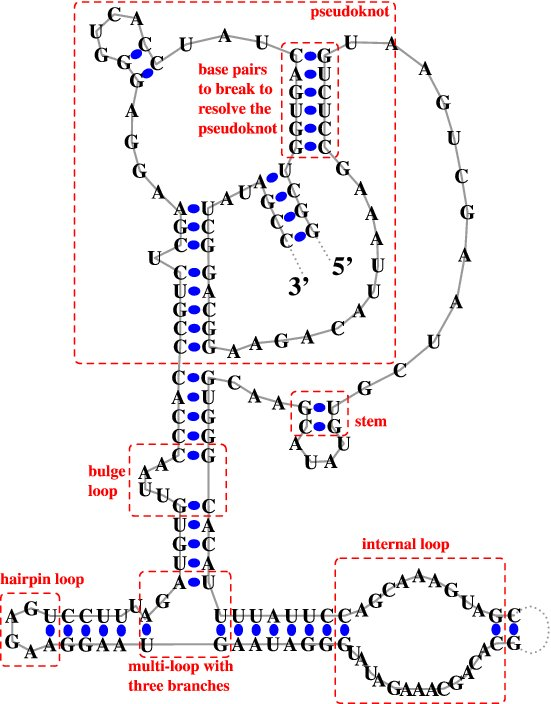
\includegraphics[width=0.7\linewidth]{secondary_structure}
	\centering
	\caption{Schematic representation of the secondary structure (a set of base pairs) for the RNase P RNA molecule of Methanococcus marapaludis from the RNase P Database. Thick blue dots represents base pairs and red dashed boxes represent structural features such as stacking, bulges, hairpin , interior, multi loops and pseduoknot structure. This figure was taken from the RNAStrand webpage.
	\label{fig:secondarystructure} 
    \citep{andronescu2008rna}}
	\end{figure}

	Single stranded nucleic acid sequences contain many complementary regions that can form double helices when the molecule is folded back onto itself. The resulting pattern of double helical stretches interspersed with loops is called the \textit{secondary} structure of an RNA.\\
	
	\section{Formal background of RNA}
	Here in this section, I would like to bring up the formal definitions of ribonucleic acid.
	\subsection{RNA Structure}
	The RNA molecules are represented as a sequence $S \in \{A, C, G, U\} ^*$.
	Formally, an RNA secondary structure $P$ of $S$ is a set of base pairs:\\
	\begin{center}
	 $ P \subseteq \{(i, j) | 1 \leq i < j \leq n $, $ Si $ and $Sj$ are complementary \},\\
	\end{center}
	where $ n = |S| $ and for all $(i, j) , ( i', j' ) \in  P:$\\
	\begin{center}
	$(i = i' \Leftrightarrow j = j')$ and $ i \neq j'$ \\
	\end{center}

	To form a valid secondary structure, the base pairs must satisfy a number of limitations. Let the bases be numbered from 1 to n in a sequence. If the bases are complementary, a base pair may form between positions $i$ and $j$ ,  if $|j - i | \geq 4$, since there must usually be at least three unpaired bases in a hairpin loop. Let bases $k$ and $l$ form another allowed pair. The pair $(k,l)$ is said to be compatible with the pair $(i,j)$ if the two pairs can be present in a structure simultaneously. Pairs are compatible if they are non-overlapping (e.g. $i<j<k<l$ ) or if one is nested within the other (e.g. $i<k<l<j$ ). The Final case, where the pairs are interlocking or crossing (e.g. $i<k<j<l$ ) is called  pseudo-knot. These pairs are assumed to be incompatible with
	most programs. An allowed secondary structure is a set of base pairs that are all compatible with each other.\\
	
	They are different types of RNA secondary structure. i.e. nested
	and crossing structures. Crossing structures contain pseudo-knots, where two structure parts overlap. Nested structures doesn't have any crossing arcs.\\
	
	\subsection{Nested secondary structure}
	Nested secondary structures can be uniquely decomposed into so called loops or secondary structure elements. Depending on the number of enclosed base pairs  and unpaired bases, different types of secondary structure elements are distinguished. These are hairpin loop, stacking, bulge loop, internal loop, multi loop. \\
	Let $S$ be a fixed sequence. Further, let $P$ be an RNA structure for $S$.
	\begin{itemize}
		\item a base pair $( i, j ) \in P$ is a \textit{hairpin} loop if\\
			$	\forall i < i' \leq j' < j : (i', j') \notin P. $

		\item a base pair $( i, j ) \in P$ is a \textit{stacking} if\\
		$(i + 1 , j - 1 ) \in P $
		\item two base pairs $ (i, j) \in P$ and $(i' ,j' ) \in P$ form  an \textit{internal} loop $(i,j,i',j')$ if \\
		$i < i' < j' < j $ ; $ (i' - i)+( j - j') > 2$ ; no base pair $(k,l)$ between $(i, j)$ and $(i',j')$
		\item An internal loop is called left (right, resp.) \textit{bulge} if\\
		$ j = j' +1 $ or $ i' = i+1$
		\item A k-\textit{multiloop} consists of multiple base pairs, $(i_1,j_1)$... $(i_k,j_k) \in P$ with a closing base pair $(j_0, i_{k+1}) \in P$ with the property that \\
		$\forall 0 \leq l \leq k : ( j_l < i_{l+1})$ ; $\forall 0 \leq l , l' \leq k$  there is no base pair $(i' ,j') \in P$ with $i' \in [j_l...i_{l+1}]$ and $j' \in [j'_l...i_{l'+1}]$ .
		\item $(i_1,j_1)...(i_k, j_k)$ are called the \textit{helices} of the multiloop.\\
 	\end{itemize}
 

 	 
 	 \subsection{Nearest neighbor model and energy contributions }
 	 
 	 \citet{DeVoe1962TheSO} said vertical stacking of bases gives largest contribution to the stability of the RNA helix. The stacking of unpaired bases is less predictable and stable than the paired bases. Hence, the directly neighboured bases must be taken into account while estimating the energy contribution of a  base pair, that results in the \textit{Nearest Neighbor Model} \citep{borer1974stability}.\\
 	 
 	 The Nearest Neighbor Model enables the calculation of a free energy estimate for a given RNA secondary structure. The free energy can be taken as the amount of energy stored in a system. The system is more stable when the energy is lower. Hence, for the \textit{most stable structure} of RNA, we go for \textit{minimum free energy (MFE)}. The energy difference between the reference state to the system is measured. We have a reference system which we use to understand the stability of the system. The reference is an RNA strcuture with no base pairing(the open chain) ie., $ E(\phi) =0 $. Hence, we need to check not only the hydrogen bonds but also the stacking stability. The Nearest Neighbor Model uses a loop-based structure decomposition. To avoid the duplication of stacking, only inner stacking are taken into account. \\
 	 
 	 \textit{The terminal mismatch} consists of the first unpaired bases immediately after the stacking. The identity of the terminal mismatch provides the energy of the loop. In Bulge or Internal loop also we have the same energy contribution. Energy contributions for external base pairs, which are not enclosed by any other base pairs, are referred to as \textit{dangling end contributions}.\\ 
 	 The energy $E(P)$ ~\ref{eq:1} of a nested secondary structure $P$ can be estimated by the sum of loop contributions (see Figure ~\ref{fig:energycontribution})\\
 	 
 	 \begin{equation}
 	 \label{eq:1}
 	 E(P) = \sum_{(i,j) \in P} \begin{cases}
 	 e^H(i,j) & : \text{if hairpin loop}, \\
 	 e^{SBI}(i,j,k,l) & : \text{if stack/bulge/internal loop} ,\\
 	 e^M(i,j,x,x') & : \text{if Multi loop},
 	 \end{cases}
 	 \end{equation}
 	 
 	 Where $e^H$, $e^{SBI}$ and $e^M$ tells the context sensitive energy contributions of the loops. $(k,l)$ represents the enclosed base pair of stack, bulge or internal and $x$ represent the unpaired bases and $x'$ represents the helices enclosed in the multi loop. We cannot see that there is an exponential number of possible multi loop composition. The energy for them can be calculated as below \\
 	 \begin{center}
 	 $e^M(i,j,x,x')= e^M_a+e^M_bx+e^M_cx'$\\
 	\end{center}
 	 where the pseudo energy parameter $e^M_a$ scores the multi loop closing base pair $(i,j)$ , $e^M_b$ represents the penalty for $x$ directly enclosed unpaired bases $x$ and $e^M_c$ scores $x'$ enclosed helices .
 	 Thus the nearest neighbor model gives the energy contributions for the loop types. \\
 	 
 	 \begin{figure}[h]
 	 	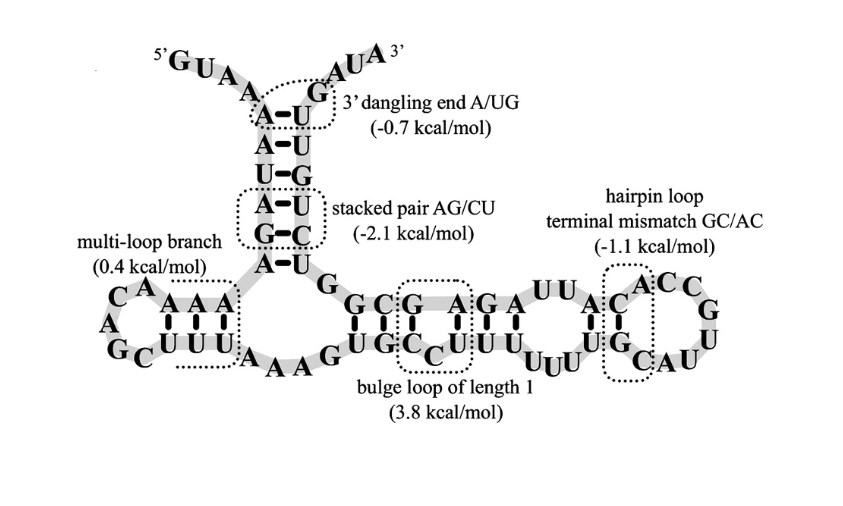
\includegraphics[width=0.9\linewidth]{energy}
 	 	\centering
 	 	\caption{Energy contributions of loops. Figure is taken from \citep{andronescu2010computational}}
 	 	\label{fig:energycontribution}
 	 \end{figure}
 	 
 	 
 	 From the above energy model, We can define a recursive dynamic programming algorithm to compute the structure which minimizes the energy function, this is called minimum free energy (mfe) structure. This algorithm was introduced by \citet{zuker1981optimal}.\\
 	 
 	 The basic substructures of the secondary structure of the RNA sequence (i.e., stack, hairpin, internal and multi loop) are independent of each other and the energy of the secondary structure is assumed to be the sum of the energies of the substructure. The algorithm is executed in two steps with a single RNA sequence as input. Firstly, the minimum free energy of the input RNA sequences is calculated, then traceback is used to recover the respective secondary structure with the base pairs. Thus given an RNA sequence $S$, Zuker’s algorithm predicts the non-crossing, minimal energy structure $P$ of $S$ in $O(n^3)$ time and $O(n^2)$ space.\\
 	 
 	 The most commonly used are the Turner parameters (\citep{mathews1999expanded}, \citep{mathews2004incorporating}) which can be found in the Nearest Neighbor Data Base NNDB. Below is the parameter sets from the Vienna RNA package.  \\
 	 
 	 For multi-loop param ( using turner 1999), the Init value is 4.1
 	 
 	 \begin{center}
 	 	A= 3.4 , B= 0.4 , C= 0\\
 	 	The stability of a 3 stem multi loop is calcualted by the equation:\\
 	 	$\triangle G = A+ B+ C $\\
 	 	A+2(B) \{loop degree of 2\}\\
 	 	therefore, the value is 4.2\\
 	 \end{center}
  
  For multi-loop param ( using turner 2004), the Init value is 4.1
  
  \begin{center}
  	A= 9.3 , B= -0.9 , C= 0\\
  	The stability of a 3 stem multi loop is calcualted by the equation:\\
  	$\triangle G = A+ B+ C  $\\
  	A+2(B) \{loop degree of 2\}\\
  	therefore, the value is 7.5\\
  \end{center}
 	 
 	 \subsection{Structure probabilities and McCaskill algorithm}
 	 Let's discuss about the structural information in terms of probabilities. According to the principal of maximum entropy \citep{jaynes1957information} the best probability distribution for the calculation of the structure or base pair probability is the \textit{Boltzmann Distribution}. These probabilities are calculated according to the Boltzmann weight. For RNA structures the unit of the energy value is $\frac{kcal}{mol}$ or $\frac{J}{mol}$. The RNA structure energy is been rescaled for Boltzmann weight computation. i.e., we replace Boltzmann constant $k_B$ with the "mol-scaled" gas constant $R$ to get the Boltzmann weight $w(P)$ of a structure $P$ as:\\
 	 
% 	 %\begin{equation*}
% 	
% 	 \begin{center}	
% 	  
% 	 \[ 
% 	 w(P)= exp\left( \frac{-E(P)}{RT} \right)
% 	 \]
% 	 \end{center}
% 	 % \label{equ1}
% 	% \end{equation*}
 	
 	\begin{equation}
 	\label{eq:equ3}
w(P)= exp\left( \frac{-E(P)}{RT} \right)
 	\end{equation}
 	 
 	 Where $E(P)$ represents the state energy, $R $ represents the gas constant and $T$ is the temperature.\\
 	 The partition function $Z$ can be calculated using the Boltzmann weights. $Z$ is the sum of the Boltzmann weights of all states within $\mathcal{P}$, which is the set of all possible structures $P$ that can be formed by $S$. \\
 	 \begin{equation}
 	 \label{eq:equ4}
 	 	%\[ 
 	 	Z= \sum_{P \in \mathcal{P}} w(P)
 	 %	\]
 		\end{equation}
 	 
 	 $Z$ is used for the calculation of structure and base pair probabilities. So in the total sum, the distribution does not change from a macroscopic point of view, therefore thermodynamic balance is reached.\\
 	 The probability of an RNA structure $P$ is given by \\ 
 	   \begin{equation}
 	  \label{eq:equ5}	 
 	 %	\[ 
 	 Pr[P|\mathcal{P}] = \frac{w(P)}{Z} 
 	 %	\]
 	\end{equation}

  	
  	 We can also calculate the probabilities of unpaired regions. Formally, we will identify the probability of the subsequences $i..j$ to be unpaired by $\mathcal{P}_{i,j}^{u}$. This probability depends on the whole ensemble of structures that can be formed by the RNA molecule of interest. Thus, it can be computed by\\
     \begin{center}	 
     	\[ 
     	\mathcal{P}_{i,j}^{u} = \frac{Z^u_{i_j}}{Z}
     	\]
     \end{center}
 	 where $Z^u_{i,j}$ is the partition function of all structures where the subsequence $i..j$ is unpaired. i.e.,\\
 	 
 	  
 	 \begin{center}	 
 	 	\[ 
 	 	Z^u_{i,j}= \sum_{P \subset \mathcal{P}_{i,j}^{u}} w(P) = Z(\mathcal{P}_{i,j}^{u})
 	 	\]
 	 \end{center}
  
  	 where $\mathcal{P}_{i,j}^{u}$ is the ensemble of all structures that are unpaired between i and j.  i.e., \\
  	 
  	 
  	 \begin{center}	 
  	 
  	 	$\mathcal{P}^u_{i,j}$= $\{P \mid \nexists (k,l) \in P\ : i \leq k \leq j $ or $ i \leq l \leq j\}\subseteq \mathcal {P}$
  	 
  	 \end{center}
  	 
  	  The calculation of accessibility of single stranded regions is carried out using  unpaired probability \citep{muckstein2006thermodynamics}, hence it is very important. 
  
 	 
 	 
 	 \begin{figure}[tb]
 	 	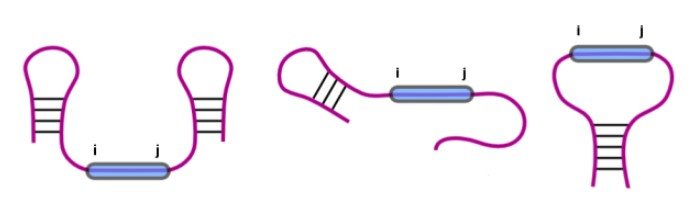
\includegraphics[width=0.8\linewidth]{unpaired}
 	 	\centering
 	 	\caption{Examplary structures that are unpaired in the subsequence {i..j}. The Figure was inspired by the lecture material of RNA bioinformatics lecture.\\}
 	 	\label{fig:unpaired}
 	 \end{figure}
  
 	 Different probabilities can be calculated using McCaskill algorithm. The McCaskill algorithm \citep{mccaskill1990equilibrium} is used to calculate the partition function $Z$ for a given sequence $S$, which can be used to compute probabilities. It enables efficient computing of the probabilities of the structure of the RNA as well as the probability that a certain base pair is formed. In addition, unpaired probabilities for subsequences can be calculated that reflect the accessibility of RNA parts for other interactions.\\ 
 	
	
	\section{RNA-RNA Interaction}
 	The interaction of RNA molecules is an essential factor for regulatory processes in all organisms. Computational prediction of RNA-RNA interactions (RRI) is a central methodology for the specific investigation of inter-molecular RNA interactions and regulatory effects of non-coding RNAs. RNA–RNA interactions are fast emerging as a major functional component in many newly discovered non-coding RNAs. They are important in many basic cellular activities including transcription, RNA processing, localization, and translation.  Many RNA species function is guided by their structure, which is defined by intramolecular base pair formation. Small prokaryotic RNAs display evolutionary unstructured regions that control the expression of their target mRNAs by intermolecular base pairing \citep{wright2013comparative}. Hence, the prediction of both functional intramolecular and intermolecular structure of RNAs are important bioinformatics tasks. \\
 	
 	Let's see about some simple RNA-RNA interactions. In \textit{splicing}, small nuclear RNA's (snRNA) can recognize intronic regions of precursor messenger RNA(mRNA) which is the important step in identifying the RNA splicing products \citep{modrek2002genomic}. In \textit{translation} transfer RNA(tRNA) interact with (mRNA) by "reading" the three letter code and define amino acid sequence \citep{selmer2006structure}, \citep{ibba2000aminoacyl}. In RNA modification, small nucleolar RNA(snoRNA) guide the modification of ribosomal RNA(rRNA) \citep{kiss2002small}. In microRNA (miRNA) targeting, the base pairing between  miRNA and mRNA leads to degradation or translation inhibition of the mRNA \citep{bartel2004micrornas}. For RNA function and regulation these examples show us the importance of the RNA-RNA interaction. \\
 		
 	In order to allow highly accurate predictions, state-of-the-art methods not only take into account the stability (energy) of possible RNA–RNA interactions, but they also consider the accessibility of the interacting subsequences \citep{umu2017comprehensive}, i.e., the intramolecular structure pattern.\\
 	
 	Small regulatory RNAs (sRNAs) typically have a range of 50 to 500 nucleotides and are transcribed through intergenic bacterial genome regions. SRNAs work in trans and display minimal complementarity with target mRNAs. They normally bind the mRNA overlapping or in the immediate vicinity of the ribosome binding site and thus affect its translation. Inhibition of translation initiation is the hybridization of the sRNA with the mRNA's 5'-UTR blocks the ribosome binding site and therefore inhibits translation initiation ~\ref{fig:srna}. \\
 	
 	
 	 \begin{figure}[tb]
 		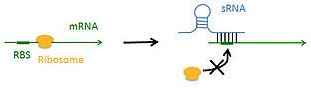
\includegraphics[width=0.8\linewidth]{srna}
 		\centering
 		\caption{sRNA translation inhibition. Figure is inspired from the site (biozentrum uni-wuerzburg)\\}
 		\label{fig:srna}
 	\end{figure}
 	
 	
 	\subsection{Formal background of RNA-RNA interactions}
 	Here, we will see the formal background of RNA-RNA interactions.\\
 	In general RNA–RNA interaction prediction (RIP) problem, given two RNA sequences $S^1$ and $S^2$ (e.g., an antisense RNA and its target), the RIP problem asks one to predict their joint secondary structure. A joint secondary structure between $S^1$ and $S^2$ is a set of “pairings” where each nucleotide of $S^1$ and $S^2$ is paired with at most one other nucleotide, either from $S^1$ or $S^2$ \citep{alkan2006rna}.  \\
 	
 	The RNA-RNA interaction is the combination of the set all of the base pairs in $S^1$, the set of all base pairs in $S^2$ and the total intermolecular base pairs between two sequences. Formally, the RRI can be modelled as RRI = $ \uplus $ bp ($S^1$) $ \cup $ $\uplus$ bp ($S^2$) $\cup$ $\uplus$ ($Inter$). Basically, the set of all base pairs of $S^1$ is $P^1$ and $S^2$ is $P^2$, then $Inter$ is $I$ which denotes the set of all intermolecular base pairs. \\
 	
 		\begin{center}
 		RRI =  $P^1$ $ \cup $  $P^2$ $\cup$ $I$
 		\end{center}
 	
 
	 	\begin{figure}[tb]
		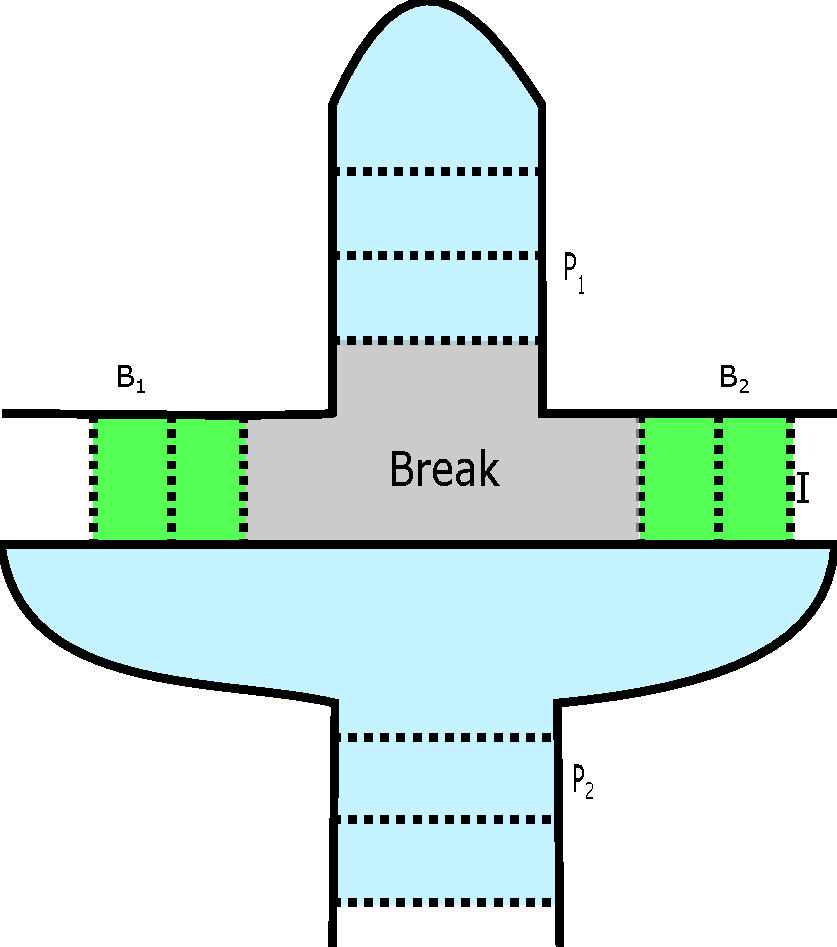
\includegraphics[width=0.4\linewidth]{rnarna.pdf}
		\centering
		\caption{The RNA-RNA Interaction is the union of all base pairs in sequence 1 and sequence 2 are denoted as $P^1$ and $P^2$ (Blue colour) respectively. $I$ (Green colour) denotes the union of all intermolecular base pairs. $B_1$, $B_2$ are the interaction blocks. Break (Grey colour) is the loop enclosed by two inter-molecular base pairs that also contains positions involved in intra-molecular base pairs}
		\label{fig:rnarna}
	\end{figure}
	
 		\begin{figure}[tb]
 		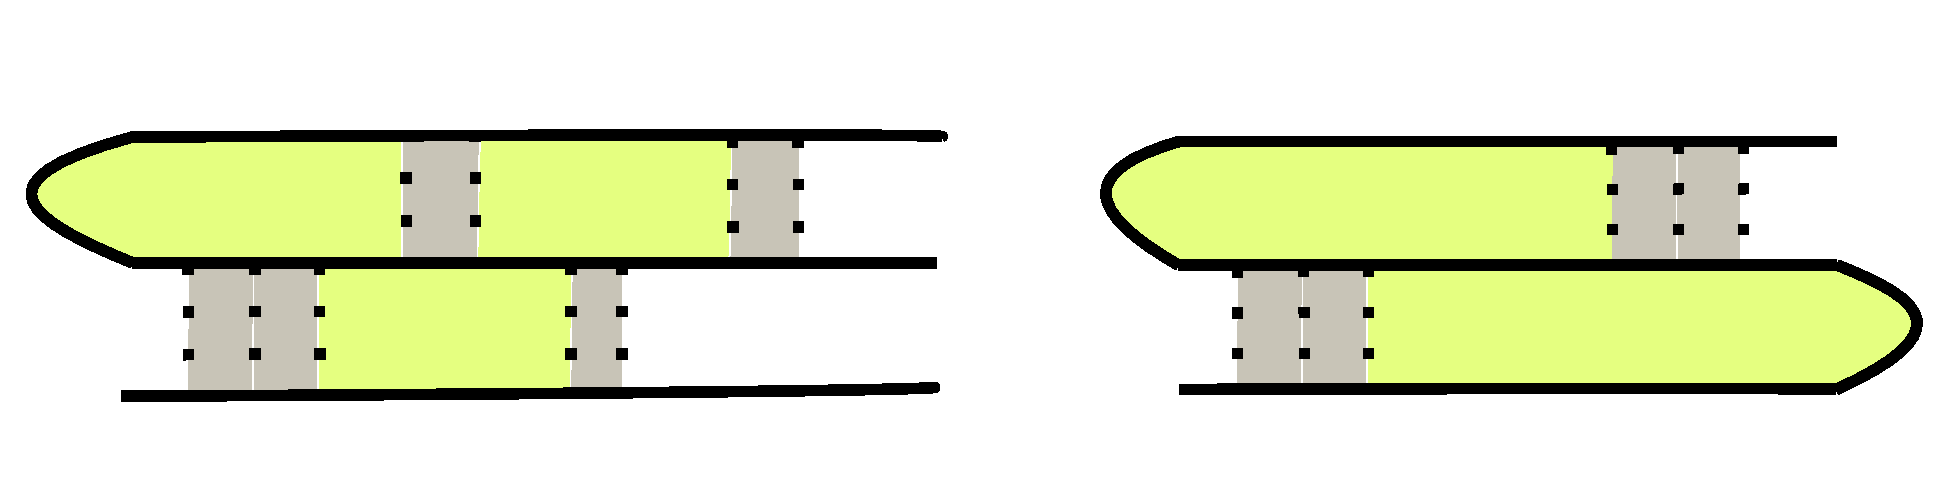
\includegraphics[width=1.0\linewidth]{pseudoknot.pdf}
 		\centering
 		\caption{ The left side figure shows the Positions are not paired within the loop. This problem starts with the pseudoknot which is shown in the right side figure where the same problem exists for the scoring of crossing structures. }
 		\label{fig:pseudoknot}
 	\end{figure}
 	
 	%The same problem we have for the scoring of crossing structure in a pseudoknot.\\
 	Now, we further decompose $I$ into the sequence of subsets of consecutive base pairs that form interaction blocks $B$ which is depicted in the Figure ~\ref{fig:rnarna}, where $ I = (B_1 ,..., B_x)$. A block $B$ is the interaction block or interaction site.
 
 	Further, the interaction block or interaction site "B" can be represented as,
 	
 	\begin{center}
 	 $B = \{ (i_1 , i_2)  \mid  S^1_{i_1}$ complementary to $ S^2_{i_2} \} \subseteq [ 1, n_1] * [1 , n_2] $
 	\end{center}
 	
 	Where for all $(i_1 ,i_2) ,(j_1, j_2) $ within a block $B$ is 
 	
 	\begin{center}
 		$(i_1 < i_2) \iff  (j_1 > j_2)$
 	\end{center}
 	
 	ie., They should be non-crossing.  The block region R(B) is $(i(B) , j(B))$ ie., left and right most base pairs of B concerning $S^1$.\\
 	
 	\begin{equation*}
 		i(B) = \argmin_{i = (i_1, i_2 ) \in B } (i_1)
 	\end{equation*}
 
 	\begin{equation*}
 			j(B) = \argmax_{i = (i_1, i_2 ) \in B} (i_1)
 	\end{equation*}
 	
 	\begin{figure}[tb]
 		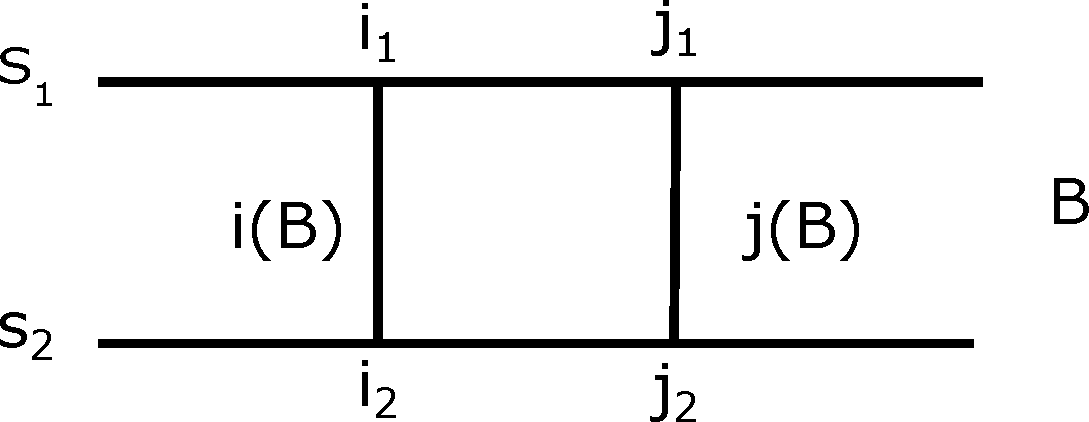
\includegraphics[width=0.6\linewidth]{block.pdf}
 		\centering
 		\caption{The block region $R(B)$ where the left and right most base pairs of $B$ concerning $S_1$}
 		\label{fig:block}
 	\end{figure}
 
 	 Furthermore, no intra molecular base pairs are allowed in block region R(B) of $P^1 , P^2$.\\
 	 ie.,
 	\begin{center}
 		 $\forall_{B\in I } : \left(\nexists_{(k,l) \in P^1} : i(B)_1 \le k \le j(B)_1  \vee   i(B)_1 \le l \le j(B)_1 \right) $ \\$\wedge $\\ 	$\left(\nexists_{(k',l') \in P^1} : i(B)_2 \le k' \le j(B)_2  \vee  i(B)_2 \le l' \le j(B)_2\right) $
 	\end{center}
 	
 	where I is the union of all blocks (ie., all inter molecular base pairs)
 	We compute the joint structure between $S_1$ and $S_2$ through minimizing their total free energy. 
	
	\begin{figure}[tb]
		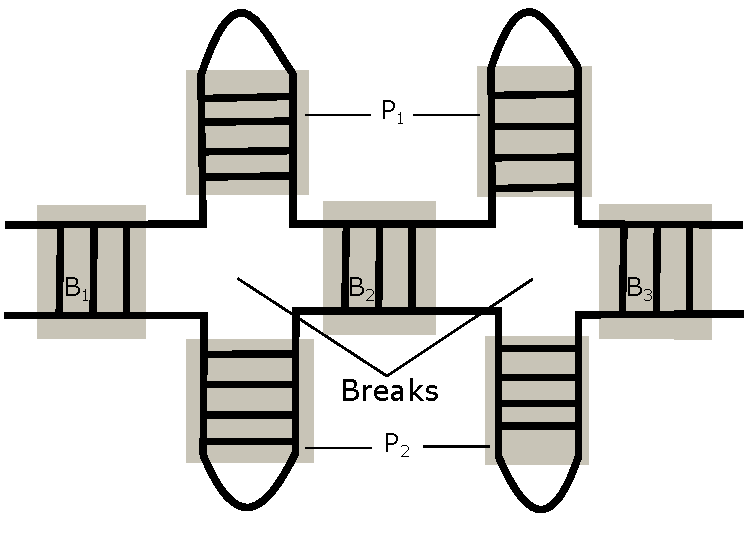
\includegraphics[width=0.5\linewidth]{break.pdf}
		\centering
		\caption{The interaction energy of RRI is the energy defined by the loops enclosed by all inter-molecular base pairs. $E(B_1)$ is the energy of block 1 and the $E(breaks)$ can be calculated from sum of all breaks.  }
		\label{fig:break}
	\end{figure}

		
	 The Energy for the block $E(B)$ can be calculated as  ,
	
%	\begin{center}
%	
%	$E(B) =  \sum_{\substack{i \in B \\ j = argmin(i') \\ i' < B \\ i'_1 > i_1}}e^{SBI}(i_1,i_2,j_1,j_2)$
%	
%		\end{center}
	
	
	\begin{equation}
	\label{eq:equ1}
	E(B) =  \sum_{\substack{i \in B \\  j = argmin(i') \\ i' < B \\ i'_1 > i_1 }}E^{SBI}(i,j,k,l)
	\end{equation}	
	
%	\begin{center}
%	$ j = \substack{argmin(i') \\ i' < B \\ i'_1 > i_1}$ 
%		\end{center}
	
%	where $j = argmin_{i' \in B \wedge i'>i}(i'_1)$. \\
	
		The $E(I)$ can be calculated as follows,
		\begin{equation}
	\label{eq:equ2}
		E(I) = E(  \uplus  B) + E_{init} 	
	\end{equation}	
	
	\begin{center}
		where, $E(  \uplus  B) = \sum_B E(B) + E(breaks)$ and $E_{init}$ is fixed init score if $I$ $\neq$ $\phi$ 
	\end{center}

	In the Fig ~\ref{fig:rnarna}, light violet colour represents the intramolecular loop with the intermolecular base pairs paired. We will need to find out, how to score them. Here, without further knowledge or energy parameters, we score it via standard loop scores ignoring the intermolecular pairings. The problem is similar to pseudoknot scoring. These also contain  the loops where the positions are not paired within the loop , see Figure ~\ref{fig:pseudoknot}.\\

	$E(breaks)$ is defined by the sum over all individual breaks between blocks (Fig  ~\ref{fig:break} ). For the $E(breaks)$ it depends on the prediction model which is a tricky part and that will be discussed with the next section along with the approaches idea. Now, we will summarise the formal definition of energy of RRI. By using the above RRI equation, we can write overall energy of RRI as \\
	
	\begin{equation}
	\label{eq:rri}
	E(RRI) = E(P^1)+E(P^2)+E_{init}+ \sum_{B_i \in I}E(B_i) + \sum_{B_i \in I} E_{break} (B_i,B_{i+1}, P^1, P^2)
	\end{equation}
	
	
	\section{RNA-RNA Interaction Prediction Approaches}
	There are several available methods, that can be classified according to their underlying prediction strategies, each implicating unique capabilities and restrictions often not transparent to the non-expert user.\\ 
	Mostly for RNA-RNA interaction prediction methods are based on thermodynamic models and provide an efficient computation since Richard Bellman’s principle of optimality \citep{raden2018interactive} can be applied. RNA–RNA interaction prediction approaches are classified into hybrid-only interaction prediction, general interaction prediction, concatenation-based/cofolding interaction prediction, and accessibility-based interaction prediction. \\
	
	In the following subsections we will see about the approaches used for predicting the RNA-RNA interactions.\\

	
	\subsection{Hybridization-only interaction prediction}
	In the hybrid-only interaction approach, the identification of RNA-RNA interaction doesn't consider intramolecular base pairs (fig ~\ref{Fig:rnahybrid}) and they can be done with $O(nm)$ time and space complexity for two RNA sequences $S^1$, $S^2$ of lengths $n$ and $m$ respectively \citep{tjaden2006target}.\\
	
	\begin{figure}[H]
		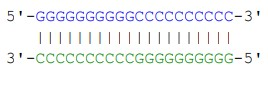
\includegraphics[width=0.4\linewidth]{rnahybrid}
		\centering
		\caption{ A full duplex structure where no intramolecular base pairs are assumed. The figure is taken from the paper \citep{wright2018structure}} 
		\label{Fig:rnahybrid}
	\end{figure}
	
	
	 A dynamic programming approach using a simplified energy model with two dimensional table H is filled via the prefix-based recursion ~\ref{eq:2}.\\
	 \begin{equation}
	 \label{eq:2}
	H_{ij} = max \begin{cases}
	H_{i-1,j-1}+1 & : \text{if $S^1_i$, $\overleftarrow{S^2_j}$ are compl. base pair }, \\
	H_{i-1,j} \\
	H_{i,j-1} ,
	\end{cases}
	\end{equation}
	Where $H_{ij}$ is the maximal number of intermolecular base pairs for the prefixes $S^1_1..i$	and $\overleftarrow{S^2_1..j}$ the reverse sequnce of $S^2$. The visual representation of the recursion scheme is given in Fig:~\ref{fig:hybrid} . The above equation is the variant of the global sequence alignment approach by \citet{needleman1970general} using scoring scheme i.e.,base pair instead of match/mismatch scoring for$S^1_i$, $\overleftarrow{S^2_j}$ no gap cost. Hence, when initialising $ H_{i,0} / H_{0,j} $ with 0, the $H_{n,m} $ gives the maximal number of intermolecular base pairs and we can trace them back. As stated above, this approach has very low runtime, which are preserved when extended to energy minimization.\\
	
	 \begin{figure}[tb]
		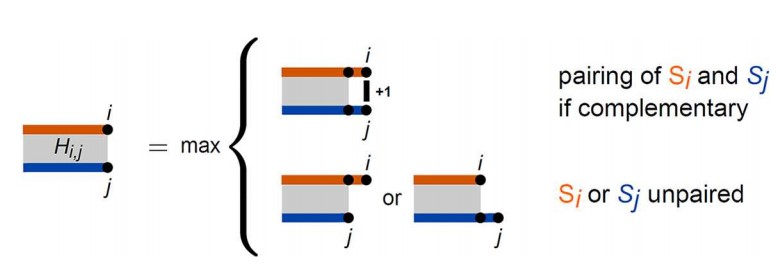
\includegraphics[width=0.8\linewidth]{hybrid}
		\centering
		\caption{Recursion scheme to maximize intermolecular base pairs between two RNAs $S1$ and $S2$ represented in orange/blue, respectively} 
		\label{fig:hybrid}
	\end{figure}

	In order to compute the energy of an RRI using ~\ref{eq:2}, no intra-molecular structure is considered, i.e. $P^1=P^2= \emptyset $ .
	
	Thus, eventually, only one block of inter-molecular base pairs is modelled ie., $(I = B)$ and no break is present. They are implemented in tools like TargetRNA, RNAhybrid. The main advantage of these approaches is they are very fast and easy to calculate the significance of hits.  Since,  intramolecular base pairing is ignored they are used for the identification of short RNA's and otherwise they overestimate the length of target sites. These disadvantages can be overcome by concatenation and accessibility based approaches.\\ 
	
	\subsection{General RNA–RNA interaction prediction}
	One of the most general approaches that is used for predicting the RRI of two intermolecular RNA molecules is IRIS \citep{pervouchine2004iris} method. This method is basically implemented by dynamic programming where it is the product of the sequence alignment and two MFOLD type secondary structure prediction algorithms. It can predict \textit{general duplex structures}. This method is applied to some well known interactions such as OxyS with fhlA mRNA which basically forms a double kissing hairpin interactions as shown Fig ~\ref{fig:doublekiss}.\\
	
	 \begin{figure}[tb]
		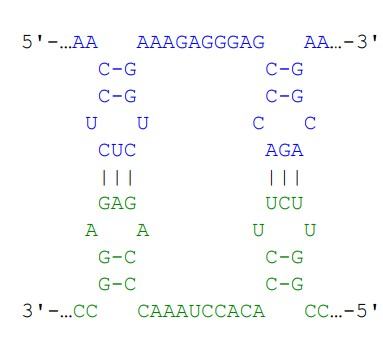
\includegraphics[width=0.4\linewidth]{doublekiss}
		\centering
		\caption{ Double kissing hairpin interaction. The blue and green denotes the first and second sequence of RNA. Base pairs are denoted by dash. The picture is taken from  } 
		\citep{wright2018structure}
		\label{fig:doublekiss}
	\end{figure}
	
	It shares most common features with pseudoknots, but is less computationally intensive. The input is made up of two sequences of RNA. Each sequence can form its own nested secondary structure and hybridize into the other molecule. The  time and space complexities are $O(n^3m^3)$ and $O(n^2m^2)$, where $n$ and $m$ are the lengths of the sequences. The configuration of the OxyS-fhlA complex proposed in \citep{argaman2000fhla} consists of four neighbouring stem loops, two in each of the molecules which connect, forming two stable kissing complexes. In this method, the main goal is the simultaneous optimization of intra- and inter-molecular base pairing.\\

	\begin{figure}[tb]
		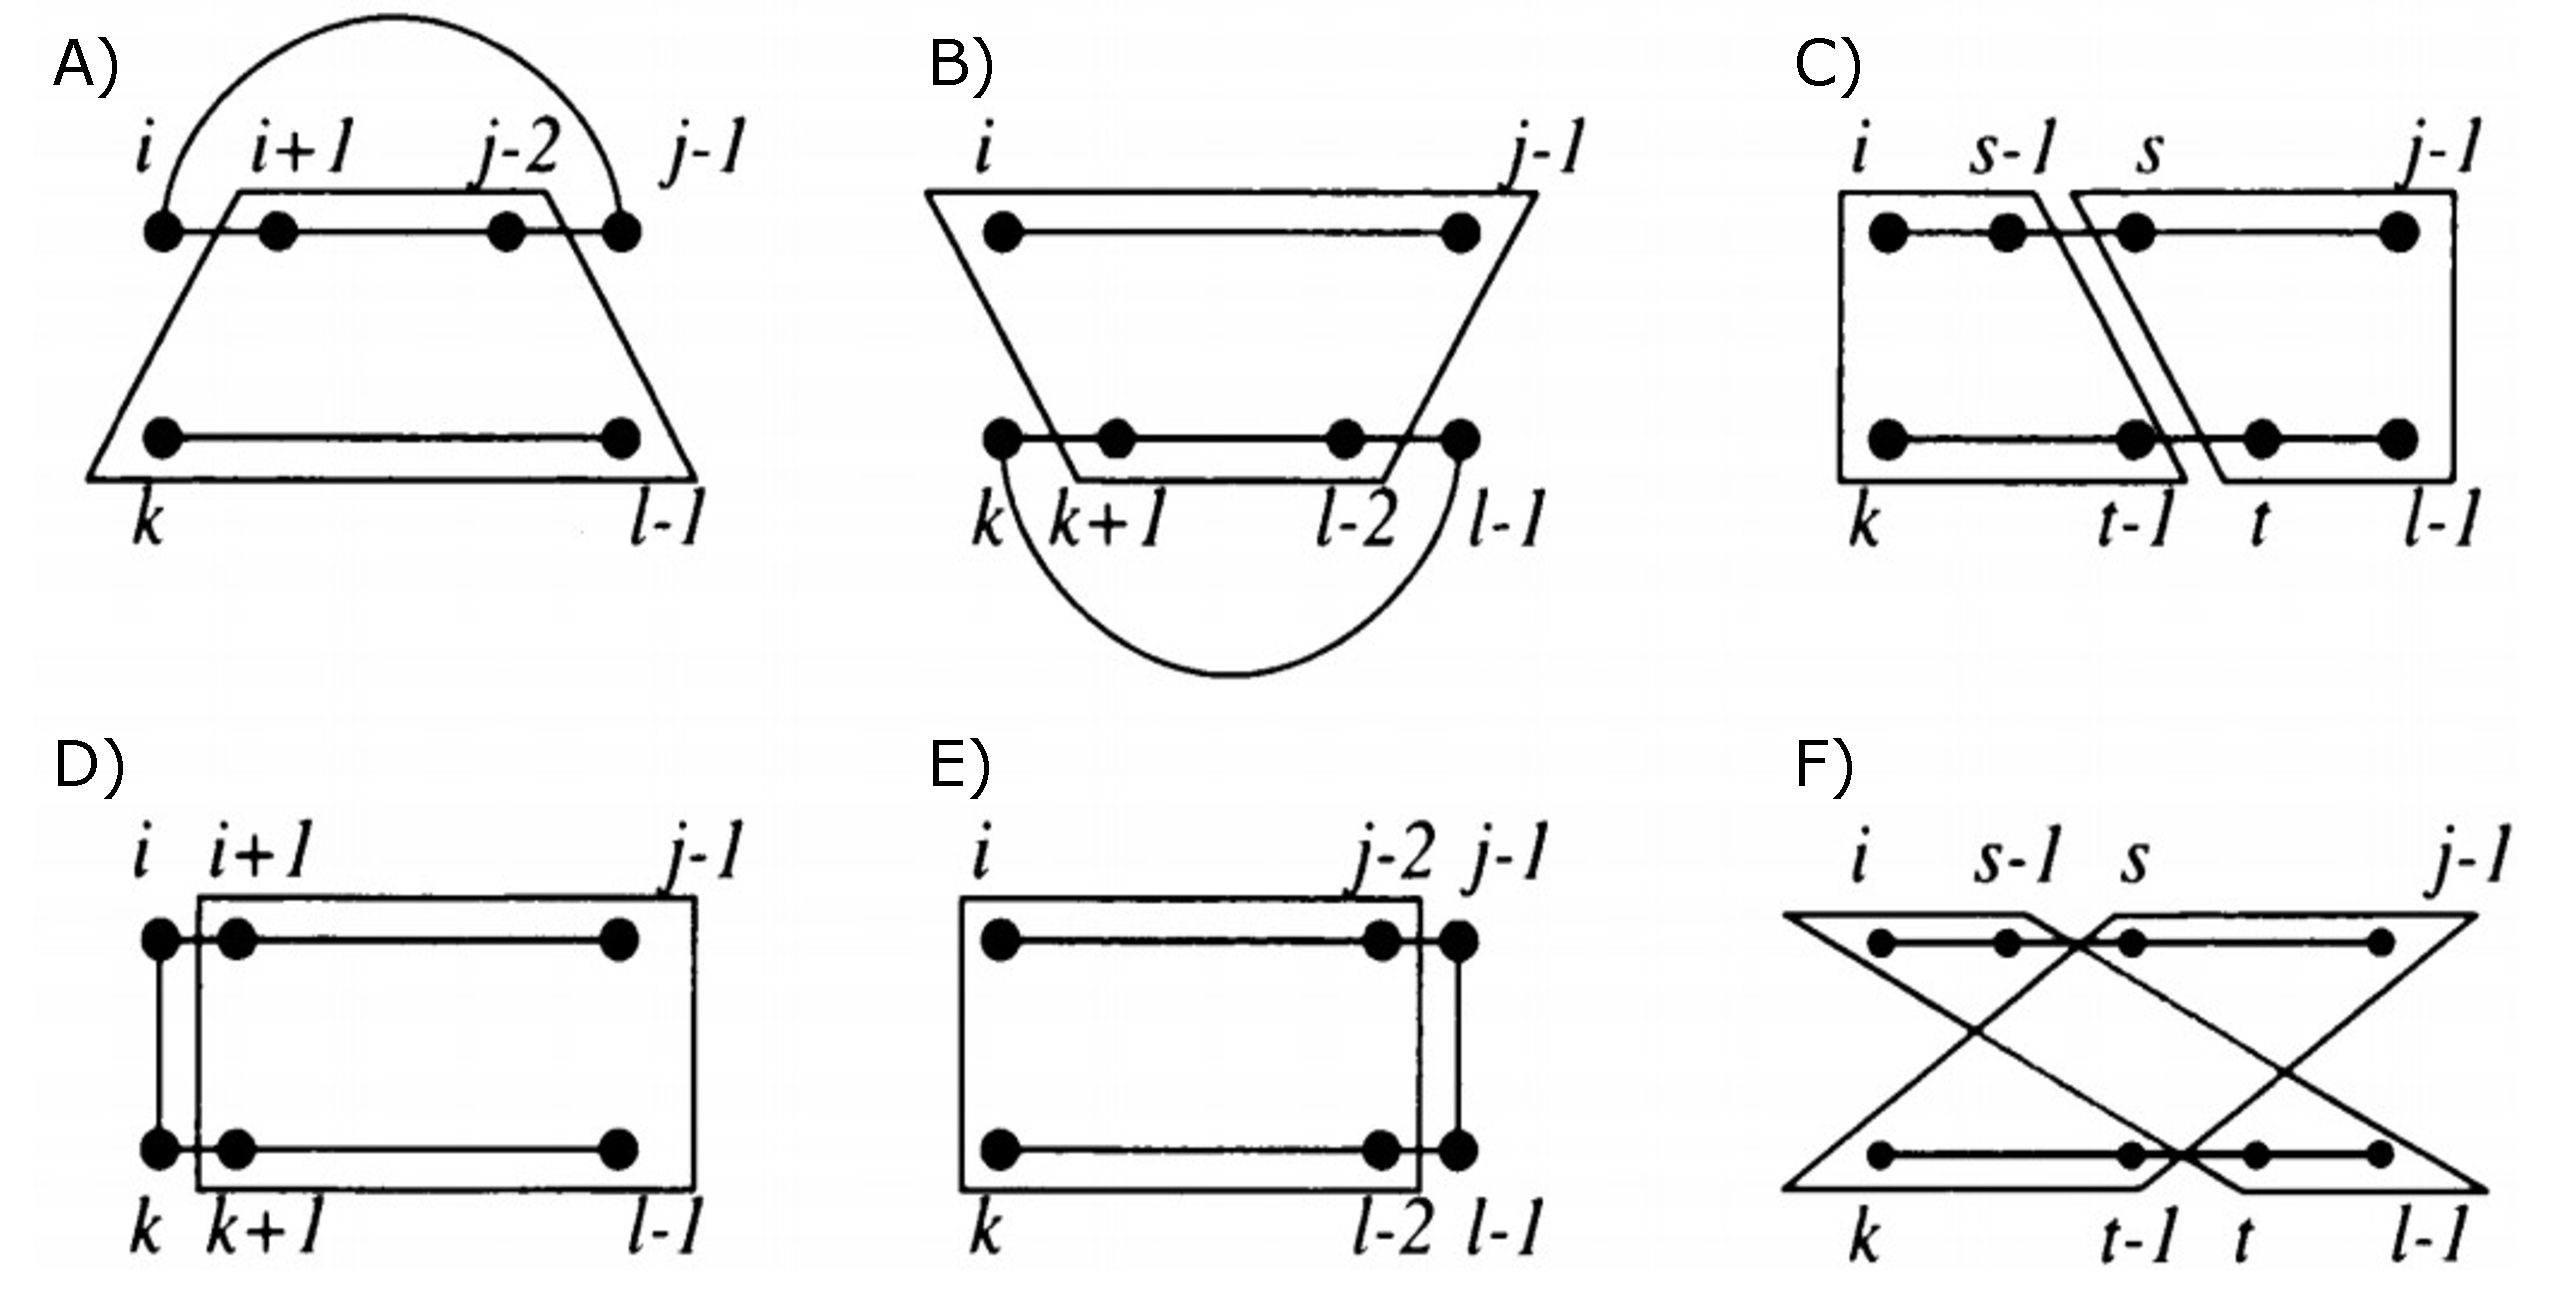
\includegraphics[width=0.9\linewidth]{iris.pdf}
		\centering
		\caption{ Depiction of the recursion $M^{i..k}_{j..l}$  which
			handles intramolecular (a,b) and intermolecular (d,e) base pair extensions as well as a general decomposition (c) and crossing (f) case.  Figure is taken from the paper \citet{pervouchine2004iris}} 
		
		\label{fig:iris}
	\end{figure}
	
	IRIS also supports crossing of consecutive blocks treated by the last recursion case in the lower right of Fig ~\ref{fig:iris}, which further complicates energy scoring of breaks. The energy contribution of general approach doesn't follow the interaction energy model instead they have pseudoknot energy. The energy associated with exterior pseudoknot can be given as \citep{xu2015physics} \\
	
		\begin{equation}
		G^{Pseudo} = \beta_1 + \beta_2 B^p + \beta_3 U^p
		\end{equation}
		
	where $\beta_1$ represents penalty for introducing a pseudoknot, $B^p$ is the number of base pairs that border the interior of the pseudoknot (i.e. number of paired positions) and $U^p$ is the number of unpaired bases inside the pseudoknot ~\ref{fig:pseudoknot}(right). If a pseudoknot is inside a multiloop then they can be represented as $\beta_1^m$( by replacing the $\beta_1$) and if pseudoknot is inside another pseudoknot they can be  represented as $\beta_1^p$ (by replacing $\beta_1$).\\
	
	As an approximation, one could use $E(PK-loop)$ with such pseudoknot energy terms based on $G^{Pseudo}$ to score breaks. Note, to get an even more accurate overall energy scoring of an interaction, one would have to use pseudoknot energy terms also for such loops formed by intra-mol base pairs (refer ~\ref{fig:pseudoknot} (left)). For simplicity, ~\ref{eq:rri} uses only nested energy terms to assess intra-molecular energies. Thus, the exact energy computation of the general approach is not covered by the formalizations used within this thesis.\\

	The time and space usage of IRIS are $ O(n^6)$ and $ O(n^4)$, respectively. The partition function version of RNA-RNA interaction prediction allows computation of probabilities of intermolecular interactions, which is used to access the stability. Due to its high complexity, several methods for reducing the requirements have been introduced. One such approach introduced by \citet{ chitsaz2009birna} called \textit{biRNA} is used to predict the multiple simultaneous binding site. \\
	
	 
	\subsection{Concatenation-based RNA-RNA interaction prediction}
	Concatenation or co-folding approach is used for predicting the interacting base pairs of two RNA molecules based on intramolecular structure prediction methods. Here,two or more sequences are concatenated  into a single sequence with special inter-spacing linker sequences. The final sequence is used within an adaptation of a standard structure prediction that takes  care of the linker sequences. \textit{mfold} was the first Concatenation-based prediction tool using the Nearest-Neighbor energy model, later implemented in \textit{MutliRNAfold} and \textit{RNAcofold}.\\

%	\begin{figure}[H]
%		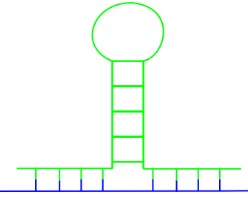
\includegraphics[width=0.3\linewidth]{concatenation}
%		\centering
%		\caption{ Green and blue are the two different RNA's that are interacting. The figure inspired from COAT PhD summer school 2012.} 
%		\label{fig:concatenation}
%	\end{figure}
	
	 RNA sequences are concatenated by a linker of length $l+1$, where l is the minimal loop size, to ensure the concatenated sequence ends can form a base pair. We don't need any special energy treatment because the intra- and inter- molecular loops are treated equally. Hence the breaks are considered as multi loop and scored accordingly. \\
		
	Concatentation-based approaches overcome the disadvantage of hybrid-only approach by incorporating the competition of intra- and intermolecular base pairing. Still they cannot predict all interaction patterns because both intra- a d inter- molecular base pairs have to be nested. For example, interactions like kissing stem-loop or kissing hairpin-loop (as seen in fig ~\ref{Fig:concat}) cannot be predicted by standard tools because they form a pseudoknot in the concatenation model. \\
	
	 \begin{figure}[tb]
		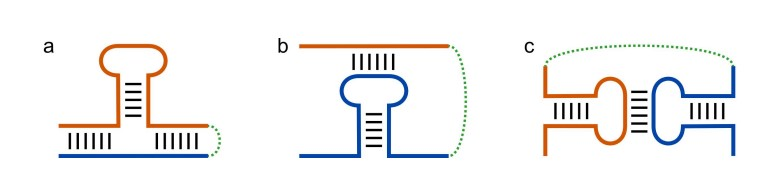
\includegraphics[width=0.9\linewidth]{concat}
		\centering
		\caption{a) Pattern that can be predicated by Concatenation b)Kissing stem-loop and c) kissing hairpin interaction. Both (b) and (c) cannot be predicted as they form a crossing structure in the concatenated model. The blue and orange are the two different RNA's and the dotted green is the linker, black lines represents the base pairs. Figure inspired from paper \citep{raden2018interactive}} 
		\label{Fig:concat}
	\end{figure}
	
	NUPACK which is a pseudoknot prediction tool that solves the problem but with the higher runtime. They are based on dynamic programming approaches for specific classes of pseudoknot structures, but does not seem to be a significant drawback in terms of the accuracy of predictions for shorter sequences. \citep{dirks2003partition}. \\
	
	\subsection{Accessibility-based interaction prediction }
	 To overcome the drawbacks of concatenation approaches, Accessibility approaches have been introduced. The main aim of this approach is to integrate ensemble properties of the single sequences that are necessary for the interaction. It can predict single site interaction patterns of two respective RNA subsequences. Tools like RNAup and IntaRNA implement this strategy. Here we have to dissolve intra molecular structure before the intermolecular interaction is formed. That is, in order to form a stable interaction of intermolecular base pairs, the intra molecular base pairs have to be opened/broken. \\
	
%	\begin{figure}[H]
%		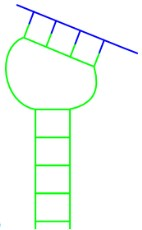
\includegraphics[width=0.2\linewidth]{acess}
%		\centering
%		\caption{ Green and blue are the two different RNA's that are interacting and forms pseudoknots. } 
%		\label{fig:acess}
%	\end{figure}

	We can classify single-site RNA-RNA interactions based on the structural context of the respective subsequences, which are\\
	
	\begin{itemize}
	\item exterior - not enclosed by any base pair.
	\item hairpin loop - directly enclosed by a base pair.
	\item non-hairpin loop - subsequence enclosed by two base pairs forming a bulge, interior or multi-loop.\\
    \end{itemize}
		
	IntaRNA can predict single-site interactions within any structural context of the respective subsequences, but concatenation-based approaches can only predict exterior-exterior context combinations. Energy scoring differs from normal $E(RRI)$, since intra-molecular structure is only considered implicitly via ensemble energies.\\
	
	The term \textit{ensemble} refers to the set of all secondary structures which can be formed through an RNA sequence. In an RNA sequence $S$, the accessibility energy of a region $[i, k]$ is determined by the energy difference (referred to as ED):
	
	 \begin{equation}
	\label{eq:equ6}
		ED(i,k) = - (E^{all} - E_{i,k}^{u} )
	\end{equation}
	
	Where $E^{all}$ denotes the energy of the set of all possible secondary structures that can be generated by sequence $S$ and $E_{i,k}^{u}$ denotes the energy of the ensemble of structures which have a single stranded area $ [i,k]$. \\
	The partition function is the total of all states $\mathcal{P}$ over the Boltzmann factors. The energy of the ensemble $E^{all}$ is 
	
	 \begin{equation}
	\label{eq:equ7}	
	E^{all} = - RTln({Z})
	\end{equation}
	The probability of unpaired regions can be used for calculating the accessibility penalty for an interval $[i,k]$, as shown below: \\
	
	\begin{align*}
	ED(i,k) &= - (E(\mathcal{P}) - E(\mathcal{P}_{i,k}^{u}))\\
	&= E(\mathcal{P}_{i,k}^{u}) - (E(\mathcal{P}) \\
	&= - RTln({Z}_{i,k}^{u}) - - RTln({Z})\\
	&= - RTln(\frac{Z^u_{i_j}}{Z})
%	&= - RTln(\mathcal{P}_{i,k}^{u})\\
	\end{align*}
	Hence,
	\begin{equation}
	\label{eq:equ10}	
	 	ED(i,k) = - RTln(\mathcal{P}_{i,k}^{u})
	 	\end{equation}
	
	 \begin{equation}
	\label{eq:equ8}	
	ED^{1}_{i,k} = - RT \cdot \log(\mathcal{P}^{u1}_{i,k})
	\end{equation}
		 \begin{equation}
	\label{eq:equ9}	
	ED^{2}_{j,l} =  - RT \cdot \log(\mathcal{P}^{u2}_{j,l})
	\end{equation}

	
	Therefore, the alternative $E(RRI)$ formula for a single interaction block B is:\\
	\begin{equation}
	E(RRI =(B)) = E(B) + E_{init} + E^{all1} + ED^1_{i_1(B),j_1(B)} + E^{all2} + ED^2{i_2(B),j_2(B)}
	\end{equation} 
	
 	Since $ED = E^u - E ^{all}$ substituting $ED$ value in  $ED + E^{all}$ gives,
	
	\begin{center}
		\[
	 E^u - E ^{all}+ E^{all}
	  = E^{u}
	  \]
	 \end{center}
	 \begin{equation}
	 \label{eq:equ11}
	 E(RRI) = E(B) + E_{init} + E^{u1} + E^{u2}
	 \end{equation}
	
	Since $E ^{all}$ is constant for a given sequence, accessibility-based approaches only optimize $(E(B) + E_{init} + ED^1_B +ED^2_B)$. To this end $P^u$ values are precomputed.\\
	
	\begin{figure}[tb]
		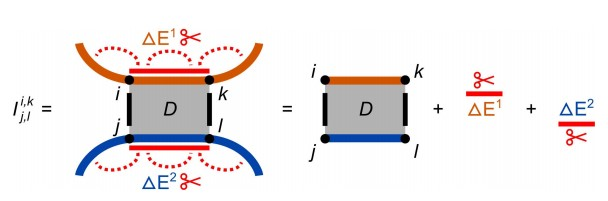
\includegraphics[width=0.9\linewidth]{access}
		\centering
		\caption{ Depiction how accessibility-based approaches score an interaction of two RNAs $S1$ and $S2$ in orange and blue respectively. $\triangle E^1 + \triangle E^2$ are the energy needed to break the intramolecular base pairs and $D$ is hybridization/duplex energy. Figure is taken from the paper \citep{raden2018interactive}} 
		\label{fig:access}
	\end{figure}
	

	The energy of accessibility approach has no break , since the interaction I forms only one interaction block. Approaches like RNAup and IntaRNA use precalculated ED values for all possible interaction regions. They gives us how much energy is needed to free of intramolecular base pairs. \\
	
		\begin{figure}[tb]
		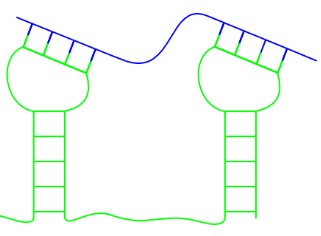
\includegraphics[width=0.4\linewidth]{doublestem}
		\centering
		\caption{ Double stem loop interaction cannot be handled by standard accessibility-based approaches as they have two binding sites (blocks) separated by intra- molecular structure. the figure is taken from COAT PhD summer school 2012} 
		\label{Fig:doublestem}
	\end{figure}
	
	
	The main drawback of accessibility approach is, it can handle only one non-crossing block. These approaches cannot be modelled correctly for the double kissing hairpin interaction which has more than one crossing blocks of interaction ~\ref{Fig:doublestem}\\
	
	
	\subsection{Comparison of approaches for RRI prediction}
	In this subsection, we will see the comparison between the approaches for some distinct interaction pattern. Below Table ~\ref{table:1} gives an overview which interaction pattern can be predicted by which approaches. \\
		\begin{table}[H]
				\caption{ Comparison of RNA-RNA interaction prediction approaches for different interaction pattern}
				\label{table:1}
		\begin{tabularx}{\textwidth}{ p{2cm}p{4.5cm}p{1.5cm}p{1cm}p{1cm}p{1cm}p{1cm} }
		\toprule
		\multicolumn{7}{c}{\textbf{Comparison of RRI approaches}}\\  
		\midrule
		\multicolumn{3}{c}{\textbf{RRI Pattern}}  & \multicolumn{4}{c}{\textbf{RRI prediction approaches}} \\
		\cmidrule(r){1-3}  \cmidrule(r){4-7}
		Figures & RRI description& No.of blocks & \rotatebox[origin=c]{90} {Hybrid-only}  &\rotatebox[origin=c]{90}{General}  &\rotatebox[origin=c]{90}{Concatenation (nested)}  &\rotatebox[origin=c]{90}{Accessibility} \\
		\hline
		\hline
		~\ref{Fig:rnahybrid}&Full duplex structure&1 &yes &yes &yes &yes\\
		\hline
		~\ref{Fig:concat} (a)& Nested joint structure without pseudoknots &2 & no &yes &yes &no \\
		\hline
		%~\ref{fig:concatenation}& Nested joint structure without pseudoknots &2 & no &yes &yes &yes \\
		%\hline
		~\ref{Fig:concat} (b)& Stem loop interaction &1 & no &yes &no &yes \\
		\hline
		%~\ref{fig:acess} & Stem loop interaction &1 & no &yes &no &yes \\
		%\hline
		~\ref{Fig:concat} (c)& Kissing hairpin loop &1 & no &yes &no &yes \\
		\hline
		~\ref{fig:doublekiss}&Double kissing hairpin loop &2 &no &yes &no &no\\
		\hline
		~\ref{fig:rnarna}& Kissing stem interaction &2 &no &yes &no &no\\
		\hline
		~\ref{Fig:doublestem}& Double kissing stem loop &2 &no &yes &no &no\\
		\hline
		\hline
		\addlinespace[0.5cm]
		NA & Best Time complexity for each \hbox{approach} & NA & $O(nm) $ & $O(n^3m^3)$ & $O(n^3)$ & $O(n^2)$ \\
	\end{tabularx}
	\end{table}

	The understanding of RNA structure and RNA-RNA interaction prediction approaches 
	is important to ensure correct result interpretation and an knowing of their limitations are necessary to avoid wrong conclusions. Here we give a concise overview of the relevant theoretical history to the most general algorithmic approaches. We could say that the accessibility-based approach is the best approach for single site RNA-RNA interaction. To handle two or multi crossing blocks of interaction, we are introducing multisite accessibility based approach. The Multi-site RRI optimization is based on single-site IntaRNA predictions. Hence, we are going for the multisite accessibility based approach in the next chapter.\\

		
		
		
	\chapter{Multisite Accessibility Based  }
	
	In this chapter, we will introduce an accessibility-based approach that can be used for multisite RNA-RNA interaction prediction. In simple words we could say, it is Multi-site RRI optimization based on single-site IntaRNA predictions. Accessibility-based RNA-RNA interaction prediction methods are typically modelling a single block of consecutive inter-molecular base pairs. Thus, interaction pattern that consists of multiple concurrently formed blocks can not be predicted. Within this thesis, we are developing and testing possibilities to efficiently predict concurrent blocks of interaction within an accessibility-based prediction model. The approach will be based on IntaRNA, which is one of the state-of-the-art programs for RNA-RNA interaction prediction.\\
	
	IntaRNA, developed by \citep{busch2008intarna} and \citep{raden2018interactive} at the bioinformatics group at Freiburg University, is a general and fast approach to the prediction of RNA-RNA interactions incorporating both the accessibility of interacting sites as well as the existence of a user-definable seed interaction. IntaRNA uses energy minimisation to find the best possible interaction.  \\
	
	Many RNAs interact via multiple synchronous, non-overlapping subinteractions (M-RRI), e.g. OxyS-fhlA. The simultaneous prediction of both intra- and inter-molecular base pairing allowing for multiple sites is computationally expensive. Current approaches include IRIS \citep{pervouchine2004iris}, NUPACK \citep{dirks2007thermodynamic},piRNA \citep{chitsaz2009partition}, etc. There are fast and reliable single interaction site (S-RRI) prediction tools like RNAup and IntaRNA, that often show the additional sites within their suboptimal list, ie. are capable of modelling all sites individually but not in a joint prediction.	To overcome this, we use the iterative method in this thesis for finding the interaction between multiple blocks. Beforehand, details of the S-RRI accessbility-based tools RNAup and IntaRNA are introduced. \\
	
	\section{RNAup - Exact Recursion for single site}
	
	In the following, I will first introduce the RNAup-like exact recursions \citep{muckstein2006thermodynamics} and then give an overview of IntaRNA heuristic version. The total energy score of the interaction is measured as the sum of the free hybridization energy and the free energy required to make the interaction sites available.\\
	
		\begin{figure}[tb]
		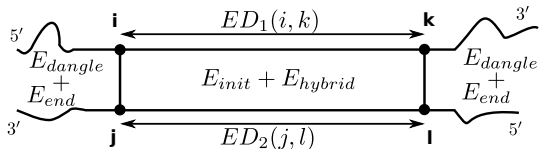
\includegraphics[width=0.6\linewidth]{inta}
		\centering
		\caption{ The energy contribution of IntaRNA. The image is taken from \citep{gelhausen2018constrained} } 
		\label{fig:inta}
	\end{figure}
	
	Thus, Scoring an interaction in IntaRNA is dependent on two energy contributions:\\
	
	\begin{itemize}
		\item \textbf{Hybridization energy} : energy value $E_hybrid$ from intermolecular base pairings in the form of stackings, bulges or internal loops, i.e., energy is typically a negative value. 
		\item \textbf{Accessibility energy} : An amount of energy  $ED $ needed to single-strand the interacting region, i.e. not include intramolecular pairings, i.e., energy is a positive value. 
	\end{itemize}
	
	
	The energy of an ensemble of structures is calculated using a partition function \citep{mccaskill1990equilibrium}. Similarly, we get $ED(i,k)$ by calculating the partition function, ${Z}_{i,k}^{u}$ covering the ensemble of all structures which can be formed by a sequence $S$, with a single stranded region $[i,k]$. As introduced in the section 1.4.4. Therefore,
	
		\begin{center}
		
		$ED(i,k) = - RTlog(\mathcal{P}_{i,k}^{u})$
		
	\end{center}
	


	\citet{muckstein2006thermodynamics} gives more detailed information on the same.
	The hybridization energy is measured using the Nearest Neighbor Energy Model. This represents the minimum free hybridization energy  of two subsequences, where a base pair is generated by the left and right most positions of both subsequences.
	For sub-sequences $S_i^1...S_k^1$ and  $S_j^2...S_l^2$ , where $S^1$ is ordered from 5' to 3' and $S^2$ in the reverse order:

%	E(B) =  \sum_{\substack{i \in B \\  j = argmin(i') \\ i' < B \\ i'_1 > i_1 }}E^{SBI}(i,j,k,l)
%	
		\begin{center}
		
%		$H(i,j,k,l) = min \{ E(P)$ | $(i, j) \in P \land (k,l) \in P \}$
		
		$H(i,j,k,l) = min_{\substack{B \\ i(B) = (i,j) \\ j(B) =(k,l)}}( E(B) )   $
		
	\end{center}
	
	The hybridization energy is calculated with a Zuker-like recursion.
	
	\begin{equation}
	\label{eq:equ12}
	H(i,j,k,l) = min \begin{cases}
	E_{init} \\
		\quad : \text{if $(S_i^1 , S_j^2 )$ can pair and $i =k , j=l $}, \\	
	min_{r,s}\{ e^{SBI}(i,j,r,s)+ H(r,s,k,l)\} \\
	 \quad 	: \text{if $(S_i^1 , S_j^2 )$ and $(S_k^1 , S_l^2)$ can pair $i < k $ and $j < l $} ,\\
	\infty \\
	\quad : \text{otherwise},
	\end{cases}
	\end{equation}
	
	Here $e^{SBI} $ is the energy contribution of stack, bulge and internal loop. The traceback helps us to find the base pairs of optimal interaction with energy $H(i,j,k,l)$. Both the accessibility and hybridisation energy forms the extended hybridisation energy which is the specific hybridisation between $S_i^1...S_k^1$ and  $S_j^2...S_l^2$ given by, 
	
		\begin{equation}
	C(i,j,k,l) =  \begin{cases}
	H(i, j, k , l) + ED_1(i, k) + ED_2(j, l) \\
	\quad 	: \text{if $(S_i^1 , S_j^2 )$ and $(S_k^1 , S_l^2)$ can pair $i \neq k $ and $j \neq l $} ,\\
	\infty \\
	\quad : \text{otherwise},
	\end{cases}
	\end{equation}
	
	We get the time and space complexity of $O(n^2m^2)$ by limiting the loop size, which is still very high. When we limit the interaction length to $l$, it has a complexity of $O(nml^2)$ time and $O(nml^2)$ space. The interaction with the minimum estimated free energy (mfe) is probably the most stable structure and thus the structure fulfills the RNA molecule function. Therefore, we are interested in \\
	
	 \begin{equation*}
	mfe = \argmin_{i,j,k,l} C(i,j,k,l)
	\end{equation*}

	
	
	\section{IntaRNA -  Heuristic recursion for single site}
	
	The exact recursions of RNAup are not suitable for larger genome wide studies due to its high time and space complexity ie., $O(n^2m^2)$	where $n$ represents the length of query and $m$ is the length of target sequence. In order to overcome the time and space complexity problem, IntaRNA introduced the heuristic recursion. This recursion is based on sparsification technique. Hence, we consider only one right end of interactions with left end $(i, j)$  which is single and locally optimal, instead of all the possible interaction. This will help us to reduce the space and time complexity to $O(nm)$, as introduced for IntaRNA version 1 \& 2. The heuristic version is defined as:
	
	\begin{equation}
	C(i,j) =  min \begin{cases}
	E_{init} + ED_1(i, i) + ED_2(j, j) \\
	\quad 	: \text{in the case of new interaction}\\
	min_{p,q}\{ e^{SBI}(i,j,p,q)+ C(p,q) - ED_1(p,K(p,q)) - ED_2(q,L(p,q))\\
	\quad \quad \quad \quad + ED_1(i,K(p,q)) + ED_2(j,L(p,q))\} \\
	\quad 	: \text{if $(S_i^1 , S_j^2 )$ can pair },\\
	\infty \\
	\quad : \text{otherwise},
	\end{cases}
	\end{equation}
	
	Here $K(p,q) , L(p,q)$ are newly introduced matrices which provide the right end of the best interaction with left end $(p,q)$. Since ED values are not additive, we have to subtract the old ED values before we add the new ED value.\\
	
	
	IntaRNA also enforces a seed region as the required constraint for the interaction of two RNAs. Seed regions are a feature found in many RNA-RNA interactions. The seed region is an interaction region of almost complete complementarity. For animal microRNAs the seed region were first discovered \citep{bentwich2005prediction}, \citep{brennecke2005principles}. Then, \citet{tjaden2006target} discovered it for many bacterial sRNAs. \\
	
	 RNAup does not use any seed condition. Within IntaRNA predictions, at least one seed is needed at the interaction site. The seed length is normally assumed to be between six and eight nucleotides. To speed up the genome-wide, methods such as RIsearch2 (\citep{alkan2017risearch2} ) or RIblast (\citep{fukunaga2017riblast} )utilize suffix-array-dependent screens to classify seed regions that are eventually expanded in both directions utilizing a predictive method focused on usability. In IntaRNA the length of the seed can be set by the user \citep{busch2008intarna}. \\
	
%	\begin{itemize}
%	
%	\item $P$: the number of bases perfectly paired in the seed region.
%	\item $b^{max} , b^{max}_m and b^{max}_s$: the maximal number of unpaired bases in the seed region.
%	
%	\end{itemize}
	
	That is, given a set of putative seed interactions $\mathcal{B}_{seed}$. We introduce additional matrix $C^{seed}$ to form a seed interaction. The seed matrix $C^{seed}$ can be filled in using the following recursion:\\
	
	
		\begin{equation}
	C^{seed}(i,j) =  min \begin{cases}
	%E_{init} + ED_1(i, i) + ED_2(j, j) \\
	%\quad 	: \text{in the case of new interaction}\\
	min_{p,q}\{ e^{SBI}(i,j,p,q)+ C^{seed}(p,q) - ED_1(p,K^{seed}(p,q)) - ED_2(q,L^{seed}(p,q))\\
	\quad \quad \quad \quad + ED_1(i,K^{seed}(p,q)) + ED_2(j,L^{seed}(p,q))\} \\
	\quad 	: \text{if $(S_i^1 , S_j^2 )$ can pair },\\
	min_{p,q}\{ seed(i,j,p,q)+ C(p,q) - ED_1(p,K(p,q)) - ED_2(q,L(p,q))\\
	\quad \quad \quad \quad + ED_1(i,K(p,q)) + ED_2(j,L(p,q))\} \\
	\quad 	: \text{if $(S_i^1 , S_j^2 )$ can pair and are left end of the seed},\\
	\infty \\
	\quad : \text{otherwise},
	\end{cases}
	\end{equation}
	
	The mfe of IntaRNA is\\
	
		
	\begin{equation*}
	mfe = \min_{i,j} C^{seed}(i,j)
	\end{equation*}
	
	
	\section{Iterative scheme for double-side RRIs}
	 In the following, we will introduce a new approach that uses a Single-RRI prediction tool (namely IntaRNA) for the prediction of Multi-RRI. For simplicity, the approach is first introduced for two sites $B_1$ and $B_2$. To this end, an iterative scheme is to be applied, which is described in the following steps.
	
	 
	 \begin{itemize}
	 	 
	
	 \item Step 1: Firstly, we have to run IntaRNA and store minimum free energy and boundaries of respective $B_1$.
	 \item Step 2: Then we get the 'blocking' constraint from step 1 to rerun IntaRNA and predict the conditional minimum free energy and site $B_2$. Here we block $B_1$ (Constrainted IntaRNA) both for intra- and inter molecular base pairing and we get $B_2$ as minimum free energy. Then, the energy of a respective M-RRI can be computed from the two energies, ie., the energy of the conditional call can be added. \\
	 \begin{center}
	 	 $E(B_1 \land B_2) = E(B_1) + E(B_2 | B_1)$ .
	 \end{center}
	 
	 \item Step 3: Since prediction of $B_2$ is conditional, the existence of $B_2$ can have effects $B_1$. Thus, one starts to iterate the procedure from (2) but swaps the conditional site and check for convergence: is the site from two-steps before retained $(B_2 == B'_2)$? If yes: convergence and stop iteration by printing the  $B_1 , B_2$. If no: repeat constraint prediction until convergence by swapping .
	 
	  \end{itemize}
  
%  	
%  	 \begin{figure}[tb]
%  		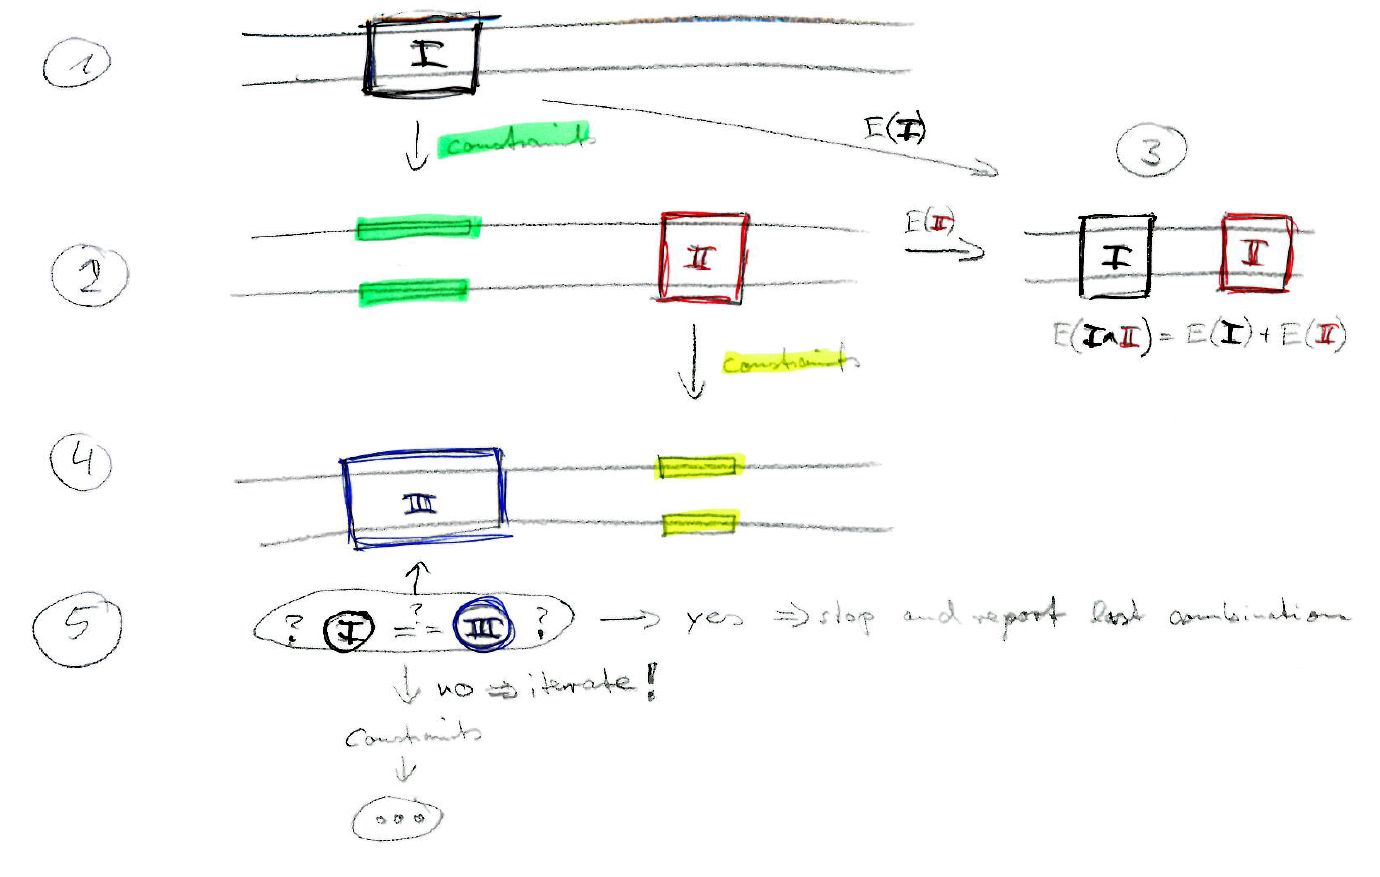
\includegraphics[width=0.9\linewidth]{idea}
%  		\centering
%  		\caption{ Iterative scheme that is used in this thesis.} 
%  		\label{fig:idea}
% 	 \end{figure}
  
  
  	Below is the flowchart representation for the same procedure.\\
	
	% Define block styles
	\tikzstyle{decision} = [diamond, draw, fill=blue!20, 
	text width=4em, text badly centered, node distance=3cm, inner sep=0pt]
	\tikzstyle{block} = [rectangle, draw, fill=blue!20, 
	text width=5em, text centered, rounded corners]
	\tikzstyle{line} = [draw, very thick, color=black!50, -latex']
	\tikzstyle{cloud} = [draw, ellipse,fill=red!20,
	minimum height=2em]
	
	\begin{tikzpicture}[scale=2, node distance = 3cm, auto]
	% Place nodes
	\node [cloud, text width=2em] (start) {start};
	\node [block, right of=start , text width=4em] (store) {$B_1$ = mfe; $B_2$ = empty};
	\node [block, right of=store, node distance=3.3cm , text width=4em] (rerun) {$B_1$ = block; $B_2'$ = mfe};
	\node [decision, right of=rerun, node distance=3.3cm, text width=3em] (decide) {$B_2$ == $B_2'$};
	\node [block, below of=decide] (swap) {$B_2$ = $B_1$ ; $B_1$ = $B_2'$};
	\node [cloud, right of=decide] (stop) {stop};
	% Draw edges
	\path [line] (start) -- node[text width=1.2cm] {run IntaRNA} (store);
	\path [line] (store) -- node[text width=1.2cm] (run) {rerun IntaRNA}(rerun);
	\path [line] (rerun) -- node[text width=1.2cm] {print $B_1$ and $B_2$}(decide);
	\path [line] (decide) -- node [near start] {yes} (stop);
	\path [line] (decide) -- node {no}(swap);
	\path [line] (swap) -| (run);
	
	\end{tikzpicture}
	
	
	Below is the proof of why the energy of the conditional call can be just added. 
	The joint site has energy \\
	
		\begin{align}	
	E(B_1 \land B_2)  \nonumber\\	
	&= E_{hyb}(B_1 \land B_2) + ED(B_1 \land B_2) \nonumber\\	
	&= E_{hyb}(B_1)+E_{hyb}(B_2)-RTlog(\mathcal{P}^u(B_1 \land B_2)) \label{1}
	\end{align}
	
	The first block $B_1$ is scored by \\
	 \begin{align}
	E(B_1) &= E_{hyb}(B_1) + ED(B_1)\nonumber\\
	&= E_{hyb}(B_1) - RTlog(\mathcal{P}^u(B_1)) \label{2}
	\end{align}
	
	and the conditional prediction of $B_2$ by\\
	
	\begin{align}
	E(B_2 | B_1) &= E_{hyb}( B_2 | B_1 )+ ED(B_2 | B_1)\nonumber \\
	& = E_{hyb}(B_2 | B_1) - RTlog(\mathcal{P}^u(B_2 | B_1)) \label{3}
	\end{align}

Now, we add right end side values of Eqn ~\ref{3} + ~\ref{2}, we get,\\
	\begin{equation}
	\label{5}
	 E_{hyb}(B_1) + E_{hyb}(B_2 | B_1) - RTlog(\mathcal{P}^u(B_1)) - RTlog(\mathcal{P}^u(B_2 | B_1))
	\end{equation}
	 
	As we know $log (A) + log (B) = log( A * B)$ , we apply this condition for log values in ~\ref{5}\\
	
	\begin{align*}
		-RTlog(\mathcal{P}^u(B_1)) - RTlog(\mathcal{P}^u(B_2 | B_1))\\
	=	-RTlog(\mathcal{P}^u(B_1) * \mathcal{P}^u(B_2 | B_1))\\
	\end{align*}
	
	Since $P(A \land B) = P(A) * P(B |A)$ and $E_{hyb}(B_2 | B_1)$ is independent of $B_1$, We get,\\
	
%	\begin{center}
%		$-RTlog(\mathcal{P}^u(B_1 \land B_2))$
%	\end{center}
%
% 	After adding and simplifying the right end side values of Eqn ~\ref{3} + ~\ref{2} we get, \\
% 	
 	\begin{equation}
 	\label{6}
 	E_{hyb}(B_1) + E_{hyb}(B_2) - RTlog(\mathcal{P}^u(B_1 \land B_2))\\
 	\end{equation}
	
	Now,  we see the equations ~\ref{6} and ~\ref{1} are equal. \\
	
	
%	\begin{equation}
%	\label{7}
%	E_{hyb}(B_1)+E_{hyb}(B_2)-RTlog(\mathcal{P}^u(B_1 \land B_2)) \Leftrightarrow E_{hyb}(B_1) + E_{hyb}(B_2) - RTlog(\mathcal{P}^u(B_1 \land B_2))
%	\end{equation}
%	
%	We also know that \\
%	\begin{align*}
%		E_{hyb}(B_1) &= E_{hyb}(B_1)\\
%		E_{hyb}( B_2 | B_1 ) &= \sum_{\forall loops in B_2}E_{hyb}(B_2)
%	\end{align*}
%	
%	Hence proved. \\
	\section{Generalization to multi-site RRI prediction}
	
	The generalized multi-site RRI prediction is similar to double-site RRI prediction. Here the process takes two steps (i) Iterative Accumulation, (ii) Iterative Refinement.\\
	 \begin{itemize}
	
	\item Step 1: Iterative Accumulation : Here, We iterate the empty list of constrained prediction and predict the minimum free energy (mfe). Every iteration returns us a list of blocks $C$. Check for mfe ($C$) exists? then, we add a new block $C=C \cup \{B_{mfe}(C)\}$. Empty list of constraints are iterated until we don't get a new block. $C' = \{C\}$. In the end, we get a list of constraints.
	\item Step 2: Iterative Refinement :For every new block (ie., $\forall b \in C$ : ($b$= $\{B_{mfe}(C \ {b})\}$), we need to check if it is restricted or not. If restricted, for all $C$, then we stop the iteration. If not, then we need to add the $C'$ to the mfe $C'$ ie.,$C=C' \cup \{mfe (C')\}$ .
	
\end{itemize}

Below is the flowchart representation for the same procedure.\\

\tikzstyle{decision} = [diamond, draw, fill=blue!20, 
text width=4em, text badly centered, node distance=3cm, inner sep=0pt]
\tikzstyle{block} = [rectangle, draw, fill=blue!20, 
text width=5em, text centered, rounded corners]
\tikzstyle{line} = [draw, very thick, color=black!50, -latex']
\tikzstyle{cloud} = [draw, ellipse,fill=red!20,
minimum height=2em]

\begin{tikzpicture}[scale=2, node distance = 1.5cm, auto]
% Place nodes
\node [cloud, text width=2em] (start) {start};
\node [block, right of=start , node distance=2.2cm, text width=3.2em] (empty) {$C$ = $\emptyset$};
\node [block, right of=empty, node distance=2.5cm , text width=4em] (iterate) {predict mfe ($C$)};
\node [decision, right of=iterate, node distance=2.8cm, text width=4.8em] (decide1) {mfe ($C$) exists ?};
\node [block, below of=decide1, node distance=3.5cm , text width=4.8em] (check1) {$C=C \cup \{B_{mfe}(C)\}$};
\node [decision, right of=decide1, node distance=3.5cm, text width=5.2em] (decide2) {$\forall b \in C$ : ($b$= $\{B_{mfe}(C \ {b})\}$};
\node [block, below of=decide2, node distance=3.5cm] (check2) {$C=C' \cup \{mfe (C')\}$};
\node [cloud, right of=decide2, node distance=3cm] (stop) {stop};
% Draw edges
\path [line] (start) -- node[text width=1cm] {empty list}(empty);
\path [line] (empty) -- node[text width=1cm] {iterate}  (iterate);
\path [line] (iterate) -- node[text width=0.5cm] {check for mfe} (decide1);
\path [line] (decide1) -- node [text width=1.5cm] {yes, add new block} (check1);
\path [line] (decide1) -- node [text width=0.7cm] (run) {no new block} (decide2);
\path [line] (decide2) -- node [text width=1.8cm] {no, $b$ not maintained } (check2);
\path [line] (decide2) -- node [text width=0.5cm] {yes for all $C$}(stop);
\path [line] (check1) -| (iterate);
\path [line] (check2) -| (run);

\end{tikzpicture}

The mfe is\\
	
			\begin{equation*}
			mfe^*(C) =  \sum_{\substack{b \in C }}(E_{hyb}(b)+E_{init}) + ED(C)
			\end{equation*}

where $ED(C)$ is $-RTlog(P_u(c))$


	\chapter{Results \& Discussion}
	
	In order to evaluate the multi site interaction, I am comparing the results of the new approach for same RNA interactions with single site interaction tool IntaRNA and results from the literature. Details of the reported RRIs are given at the end of the section in ~\ref{table:2} \\ 
	
	
	\section{Setup}
	
	I have used the IntaRNA-3.1.3-windows-64bit version for my thesis. The following parameter has been set. The --outMode=C a flexible interface to generate RNA-RNA interaction output in CSV format (using ; as separator). The argument -n 1 or --outNumber=1 can be used to generate up to N interactions for each query-target pair. IntaRNA provides the possibility to constrain the accessibility computation using the --qAccConstr and --tAccConstr parameters. In this I have used "b" blocked to indicate the positions are occupied by some other interaction (implies single-strandedness). It is possible to restrict the overall length an interaction is allowed to have. This can be done independently for the query and target sequence using --qIntLenMax and --tIntLenMax, respectively. We can alter indexing (independently for query and target) using the --qIdxPos0 and --tIdxPos0 parameters, respectively. Here, the overall energy E has times of $E_{init}$.\\
	
	
	With the above setup, we were able to test multi-site RNA-RNA interactions. The used sequences are listed in Appendix Table.\\
	
%	\begin{table}[h]
%		\centering
%		\csvautotabular{datacollection.csv}
%		\caption{ Collections of multisite RNA interaction}
%	\end{table}
%	
	
		
		
%	\begin{figure}
%		\centering
%		\begin{subfigure}{.5\textwidth}
%			\centering
%			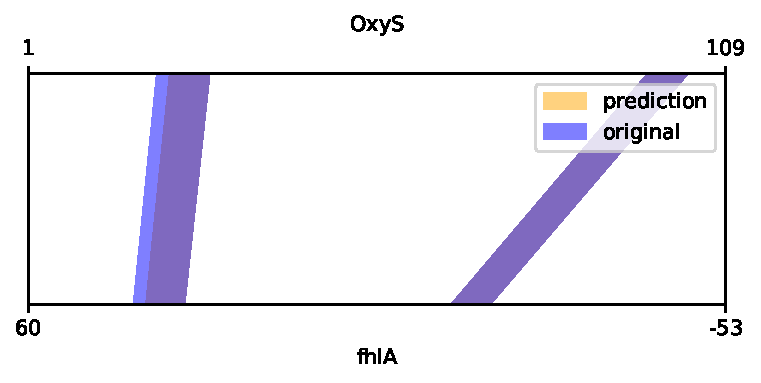
\includegraphics[width=0.9\linewidth]{rricomparison1.pdf}
%			\caption{OxyS:fhlA}
%			\label{fig:rricomparison1}
%		\end{subfigure}%
%		\begin{subfigure}{.5\textwidth}
%			\centering
%			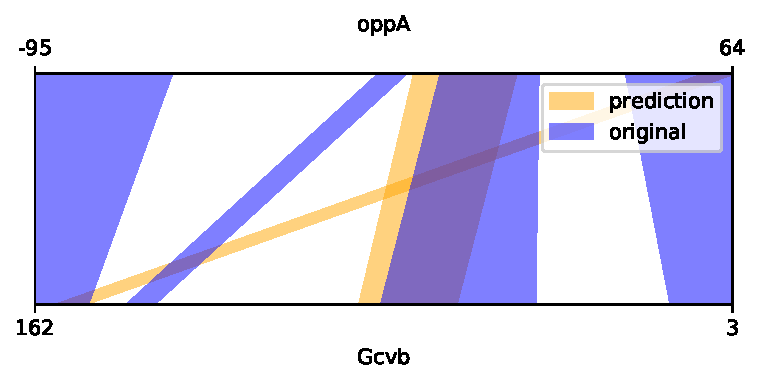
\includegraphics[width=.9\linewidth]{rricomparison6}
%			\caption{oppA:Gcvb}
%			\label{fig:rricomparison6}
%		\end{subfigure}
%		\begin{subfigure}{.5\textwidth}
%			\centering
%			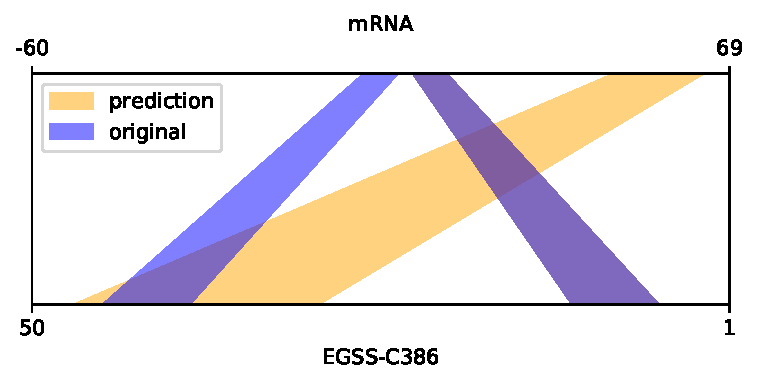
\includegraphics[width=.9\linewidth]{rricomparison4}
%			\caption{mRNA:EGS S-C386}
%			\label{fig:rricomparison4}
%		\end{subfigure}%
%		\begin{subfigure}{.5\textwidth}
%			\centering
%			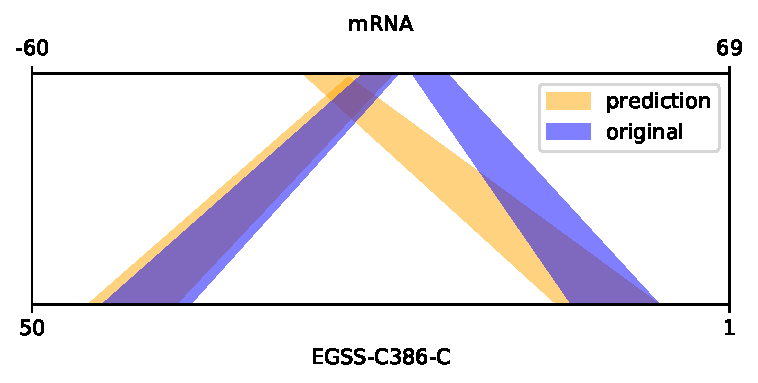
\includegraphics[width=.9\linewidth]{rricomparison5}
%			\caption{mRNA:EGS S-C386-C}
%			\label{fig:rricomparison5}
%		\end{subfigure}
%		\begin{subfigure}{.5\textwidth}
%			\centering
%			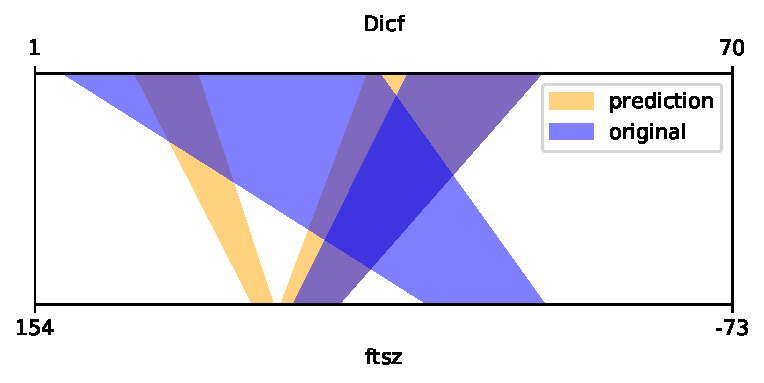
\includegraphics[width=.9\linewidth]{rricomparison3}
%			\caption{Dicf:ftsz}
%			\label{fig:rricomparison3}
%		\end{subfigure}%
%	\begin{subfigure}{.5\textwidth}
%		\centering
%		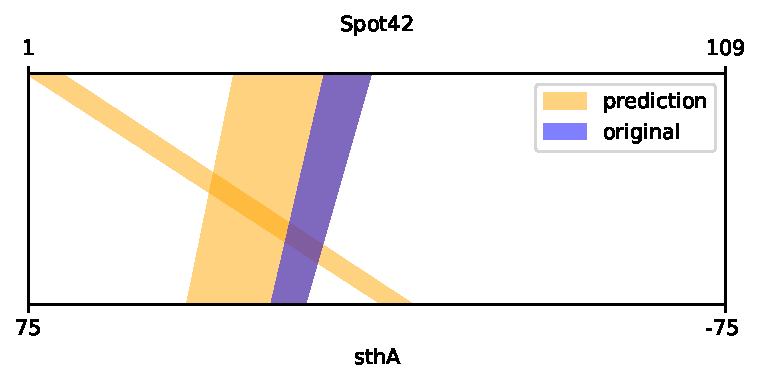
\includegraphics[width=.9\linewidth]{rricomparison2}
%		\caption{spot42:stha}
%		\label{fig:rricomparison2}
%	\end{subfigure}
%\begin{subfigure}{.5\textwidth}
%	\centering
%	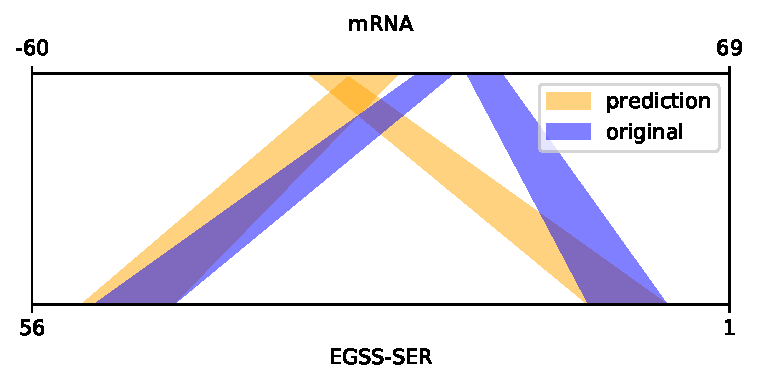
\includegraphics[width=.9\linewidth]{rricomparison7}
%	\caption{mRNA:EGS S-SER}
%	\label{fig:rricomparison7}
%\end{subfigure}%
%\begin{subfigure}{.5\textwidth}
%	\centering
%	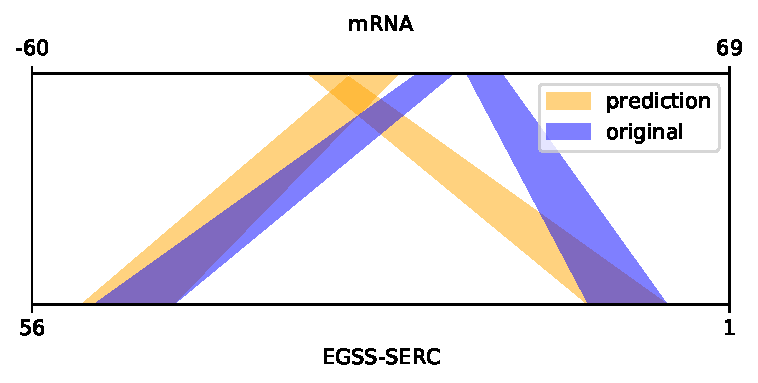
\includegraphics[width=.9\linewidth]{rricomparison8}
%	\caption{mRNA:EGS S-SERC}
%	\label{fig:rricomparison8}
%\end{subfigure}%
%
%		\caption{Multisite Interaction prediction for various RNA's}
%		\label{fig:test}
%			
%	\end{figure}

	
	\section{OxyS – fhlA}
	
	The small RNA OxyS binds to a short sequence inside the fhlA mRNA coding region. This is one of the classic examples of multi-site RRI where OxyS forms a stable kissing hairpin complex with fhlA. \\
	Details of the interaction are taken from the paper ~\citep{argaman2000fhla}. The pairing mechanism between the two RNAs is dramatically influenced by their structure. For this purpose, a full comprehension of the pairing process involves thorough knowledge of the individual RNA structures. \\
	
	When OxyS binds fhlA mRNA it forms kissing complex structure and results in a healthy anti-sense-target structure. The secondary structure of the 5' end region of fhlA mRNA was predicted to include two stem loop structures. The findings of the study of the structure confirm the presence of the two structure. \\
	
	When we run with IntaRNA first, we observed that the OxyS (98 - 104) interacts with fhlA (-9 - -15), ie.,104:-15\& 98:-9 is the block that is predicted with the energy -4.37. Then, we run them with our tool, the total energy for both blocks is -7.99. Here the sequence length for OxyS starts from 1 to 109 and for fhla it is from -53 to 60. We can clearly see from the Fig ~\ref{fig:rricomparison1} where the predicted interaction (orange) and the original (blue) interaction from the paper interacts almost at the same place. \\
	


	\begin{figure}[h!tb]
	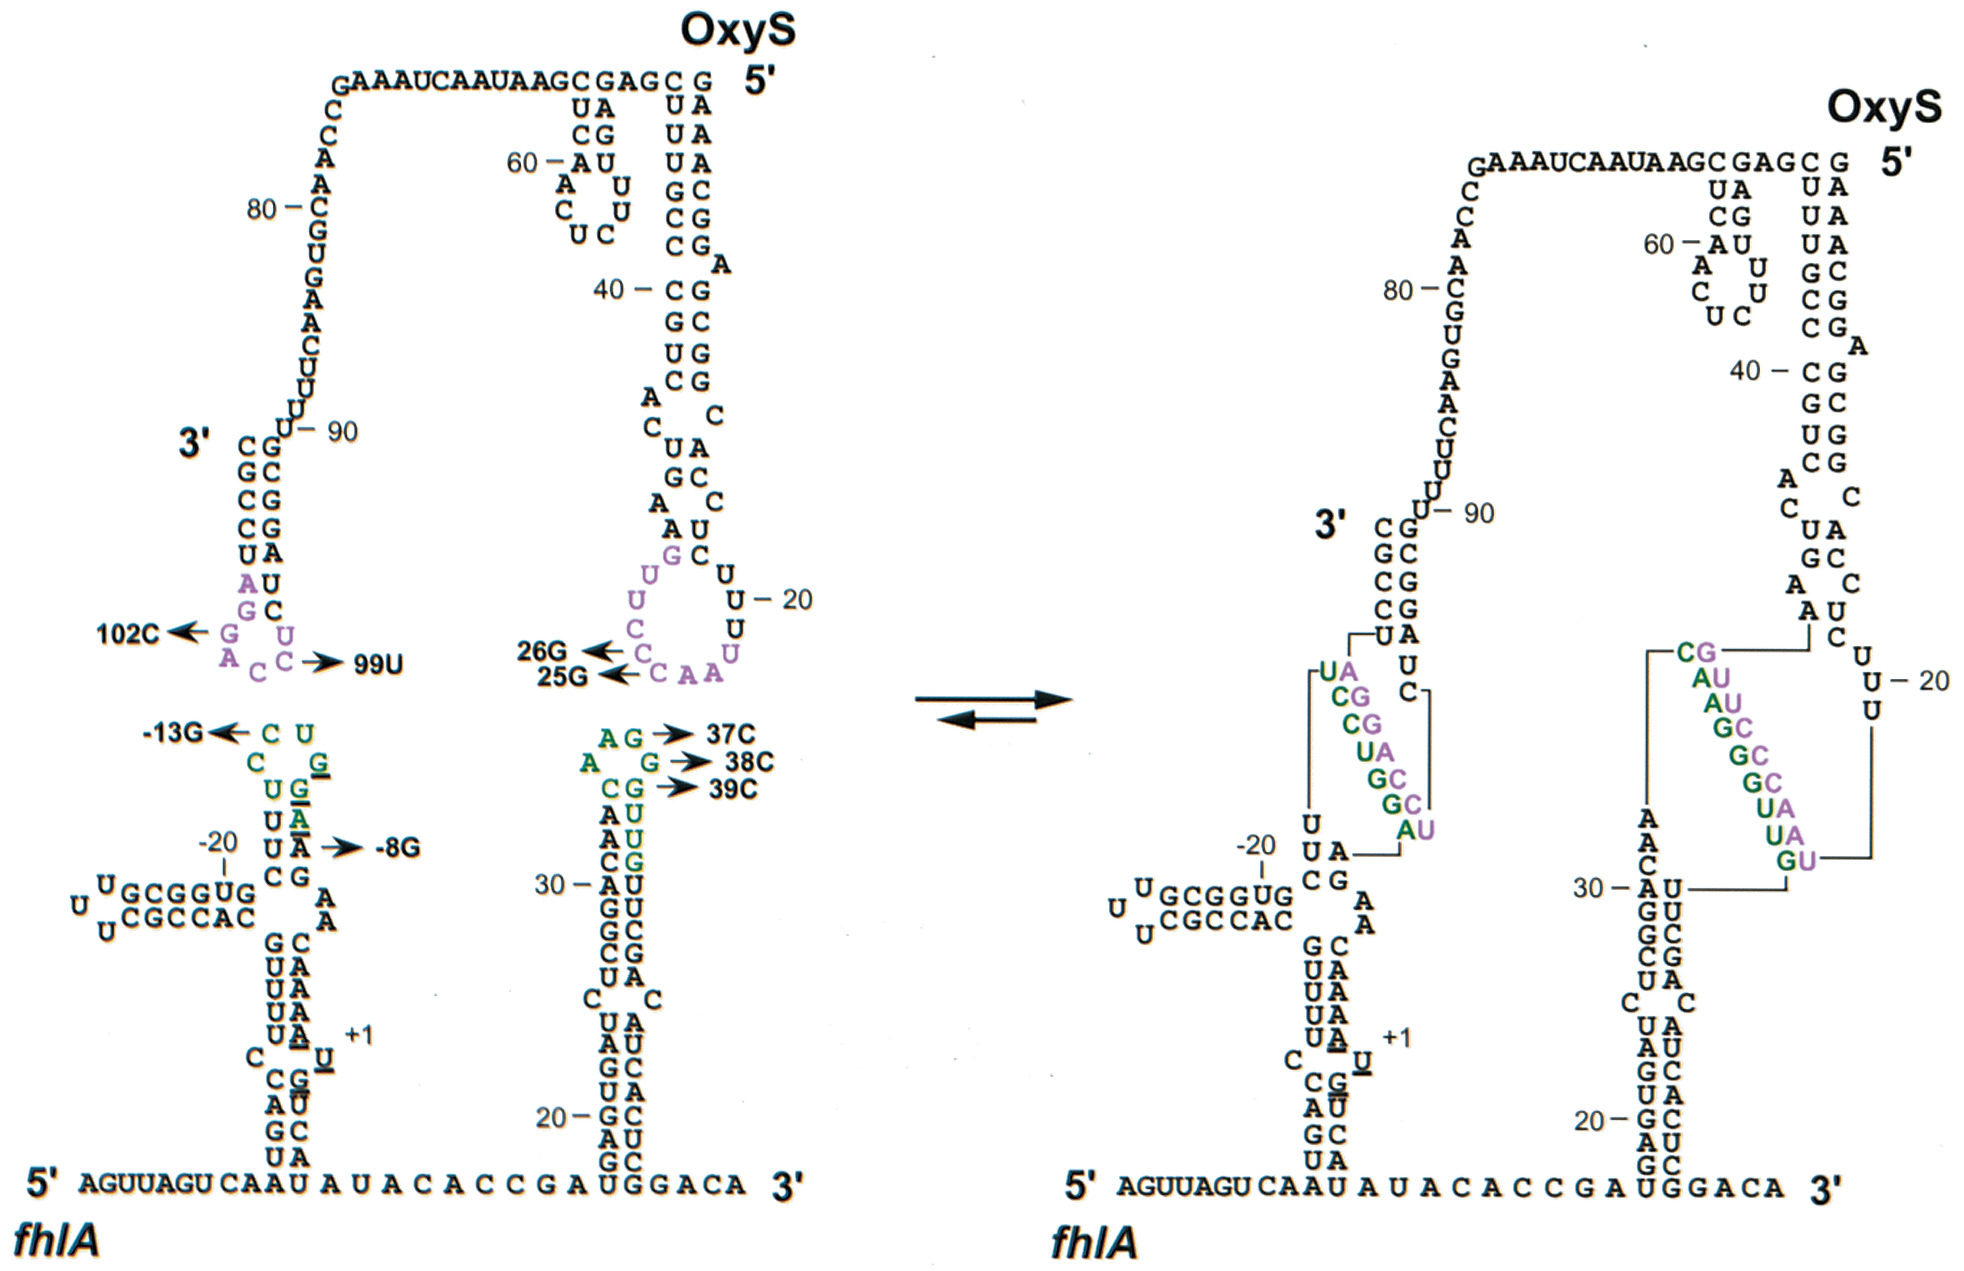
\includegraphics[width=1.0\linewidth]{oxys}
	\centering
	\caption{ Interaction of OxyS - fhlA. The numbering of fhlA begins with the initiation codon (AUG). The counting of OxyS begins at the transcription start site. Figure is taken from \citep{argaman2000fhla}. } 
	\label{fig:oxys}
	\end{figure}

\begin{figure}[h!tb]
	\centering
	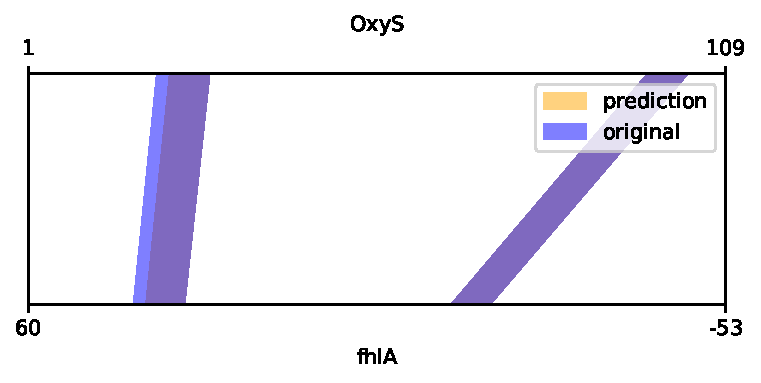
\includegraphics[width=.4\linewidth]{rricomparison1.pdf}
	\caption{OxyS:fhlA interaction that is predicted using double-site tool. We can see that predicted interaction (orange colour) is highly similar to the original interaction (blue colour). }
	\label{fig:rricomparison1}
\end{figure}

\clearpage
	
	
	
	\section{Spot42 – sthA }
	
	The next interesting example is Spot42 interaction with sthA. The RNA Spot42 plays a large role in the suppression of catabolites in Escherichia coli (E.coli) by the direct suppression of genes involved in primary and secondary metabolism.\\
	
	This example is taken from \citep{beisel2011base}. Spot42 is interacting with its targets via three conserved accessible regions (I – III) refer to left side Fig ~\ref{fig:be} . \\
%	To validate base pairing through the three single-stranded regions II of Spot 42, compensatory mutations have been made in sthA. Such findings suggest that the base pairing with target mRNAs can accrue at three single-stranded regions of Spot 42. \\
	The mutation in region III influenced the repression of fusion of sthA the most (refer right side Fig ~\ref{fig:bei2} ). Mutating sites I and III were reported to have the highest impact while Region II mutation showed only slight effects. It has been shown that mainly sites I and III are important for the interaction with the target mRNA encoded by the sthA gene. This suggests multiple interaction possibilities of Spot42 with sthA, as discussed in  ~\citet{mann2017intarna}.\\
	
	 The graph in the Figure ~\ref{fig:be} never shown zero because there is always a some part of mRNA still interacts and we get amount of protein formation. In hypothesis, we say that if we mutate two sides I and III, we get the full repression.\\
	
	
	
	
	 \begin{figure}[h!tb]
		\centering
		\begin{subfigure}{.5\textwidth}
			\centering
			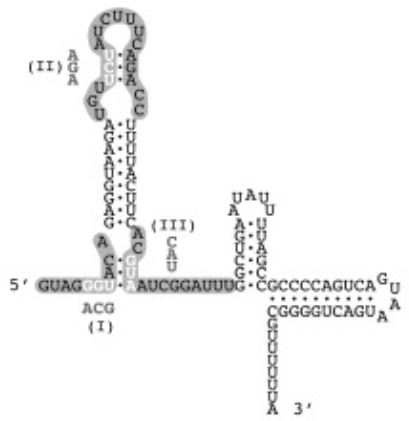
\includegraphics[width=.9\linewidth]{bei}		
			\label{fig:bei}
		\end{subfigure}%
		\begin{subfigure}{.5\textwidth}
			\centering
			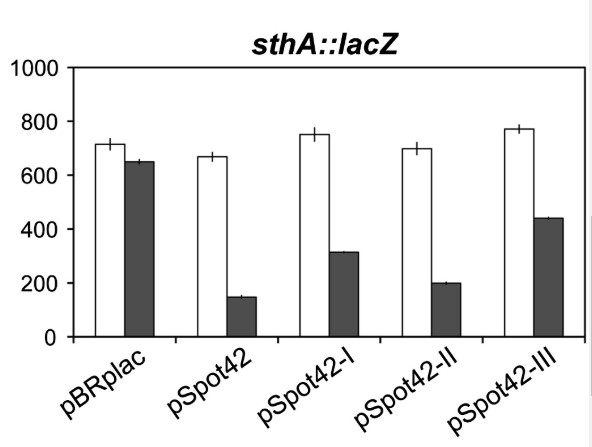
\includegraphics[width=.8\linewidth]{spot42}	
			\label{fig:spot42}
		\end{subfigure}
	\caption{ The left side of the figure shows the secondary structure of Spot 42. Mutated regions are in grey colour. Right side of the figure shows the mutational analysis of base-pairing interactions of Spot42 – sthA. Spot 42 base pairs directly with target genes via three separate regions is shown. Figure is taken from the paper \citep{beisel2011base}. The black bar shows the translation product measure of sthA gene and the white one is a control molecule to compare for the different experiments (translational reference). }
	\label{fig:be}
\end{figure}
	
%		\begin{figure}[h!tb]
%		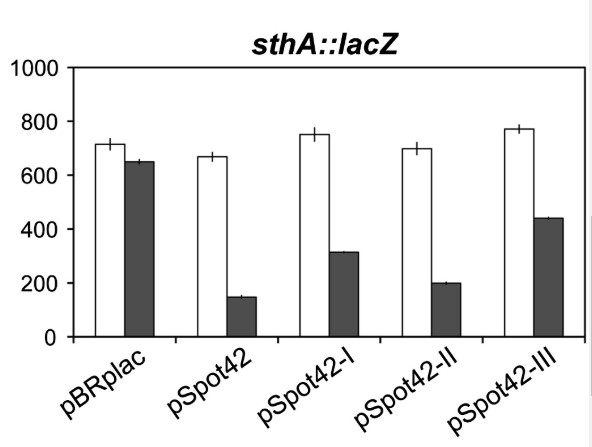
\includegraphics[width=0.6\linewidth]{spot42}
%		\centering
%		\caption{ Mutational analysis of base-pairing interactions of Spot42 – sthA. Spot 42 base pairs directly with target genes via three separate regions is shown. Figure is taken from the paper \citep{beisel2011base}  } 
%		\label{fig:spot42}
%	\end{figure}

%	\begin{figure}[h!tb]
%		\centering
%		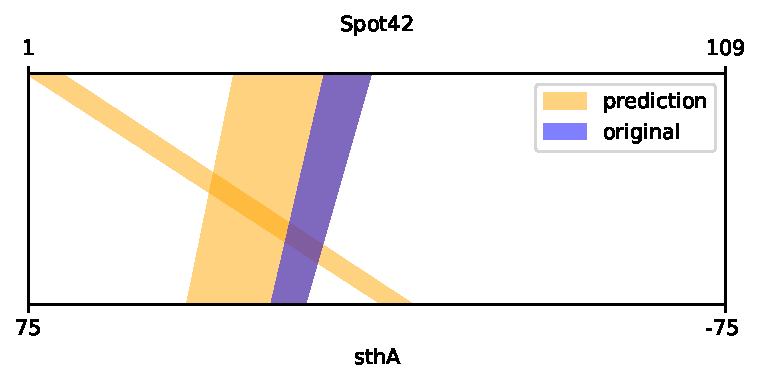
\includegraphics[width=.5\linewidth]{rricomparison2}
%		\caption{spot42:stha interaction that is predicted using double-site tool. We can see that predicted interaction (orange colour) of two blocks and single original interaction block(blue colour).  }
%		\label{fig:rricomparison2}
%	\end{figure}

 \begin{figure}[h!tb]
	\centering
	\begin{subfigure}{.5\textwidth}
		\centering
		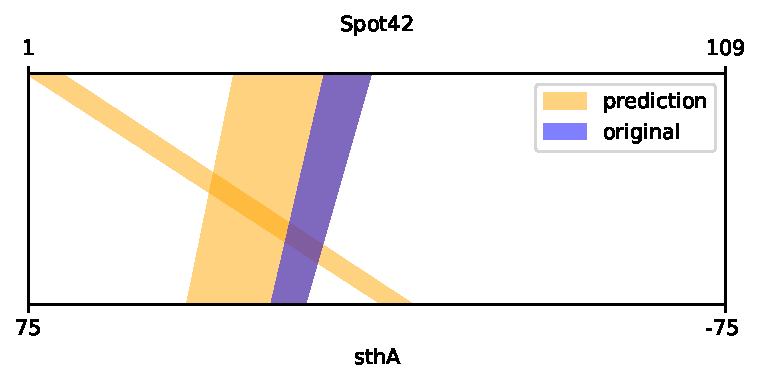
\includegraphics[width=1.0\linewidth]{rricomparison2}		
		\label{fig:rricomparison2}
	\end{subfigure}%
	\begin{subfigure}{.5\textwidth}
		\centering
		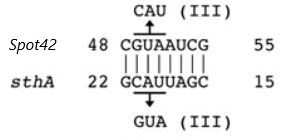
\includegraphics[width=.8\linewidth]{bei0}	
		\label{fig:bei0}
	\end{subfigure}
\caption{ The left side of the figures shows the Spot42:sthA interaction that is predicted using double-site tool. We can see that predicted interaction (orange colour) of two blocks and only one original interaction block(blue colour) of original is shown as the other interaction is not given in the literature.  The right side of the figure shows the base-pairing interactions with Spot 42 predicted by the folding algorithm NUPACK. Mutation in Region III is shown. Figure is taken from the paper \citep{beisel2011base}  }
\label{fig:bei2}
\end{figure}

When we run with IntaRNA first, we observed that the Spot42 (34 - 55) interacts with sthA (15 - 40), ie.,55:15\&34:40 is the block that is predicted which refers to region III and the mfe is -7.85. Then, we run them with our tool here when Spot42 interacts with sthA, we observed that the total energy value is -26.38. The prediction provides a model for the concurrent interaction of region I and III. If we need to have the same ED values, then we can use the --energyNoDangles option. Here for Spot42, we couldn't find the original interaction, hence we are comparing with the bar chart from the figure 2 from paper {\citep{beisel2011base}}. From the right side figure ~\ref{fig:be}, we can clearly see, mutating sites I and III showed the highest effect while region II mutation showed only small effects. This is because, I and III are close in structure though they are far away from the sequence.\\

\clearpage

	\section{GcvB – oppA }
    The gcvB gene encodes two small, nontranslated RNAs that regulate oppA. The structure of the GcvB-oppA complex consists of two intermolecular helices that precede and follow the putative terminator. This is an example where there are four concurrent blocks predicted by the IRIS tool {\citep{pervouchine2004iris}}. \\ 
    
     oppA is the periplasmic-binding protein portion of the OppABCDF oligopeptide transport system. The functional consequence of deleting the gcvB gene is a derepression of oppA. The mechanism of GcvB regulation of oppA is likely to be on a translational level \citep{urbanowski2000gcvb}. One of the major role of oppA is the transport of dietary peptides.\\
    
    Study of the GcvB sequence identified a complementarity area near the ribosome-binding sites of oppA mRNAs. The findings from {\citep{pulvermacher2008role}} indicate that various regions of GcvB have specific functions in the control of oppA mRNA. The Shine-Dalgarno sequence in the GcvB-oppA complex is obstructed ~\citep{pervouchine2004iris} and the complex structure is located in the upstream region. This is very much in accordance with the assumption that the oppA control seems to be at the translational stage. \\
    
    When we run with IntaRNA first, we observed that the oppA (-9 - 14) interacts with GcvB (67 - 89), ie., 14:67\&-9:89 is the block that is predicted with an mfe of -14.57. Then, we run them with our tool as, we predict the double block interaction, we have predicted the two sites of the interaction out of four. The total interaction energy for two sides of block is 26.38 kcal/mol. Also, in the prediction we get a crossing structure, which is in contrast to the model by IRIS , Fig :~\ref{fig:oppa}. Second block NOT in accordance with IRIS prediction. \\
	
		\begin{figure}[h!tb]
		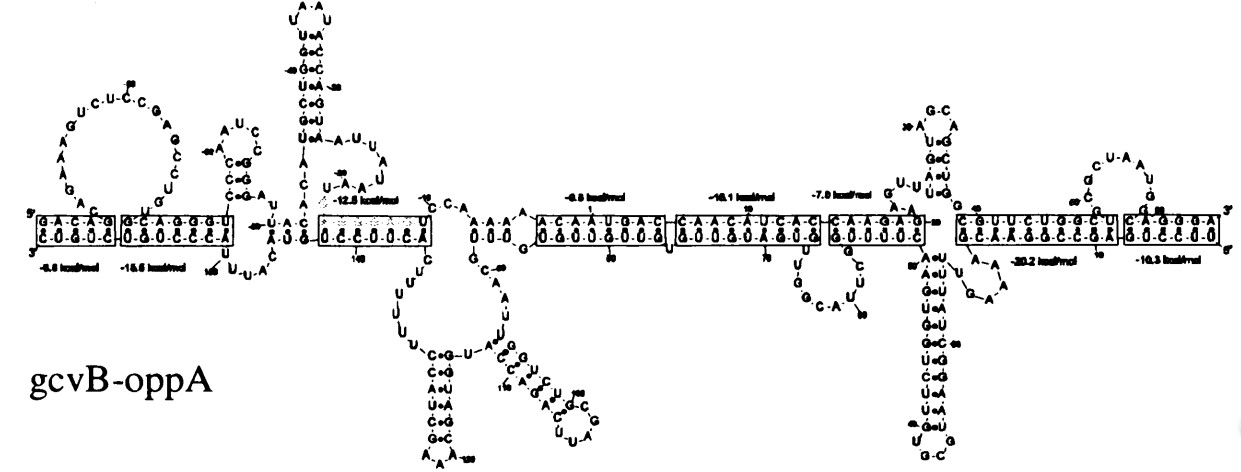
\includegraphics[width=1.0\linewidth]{oppa}
		\centering
		\caption{ Interaction of GcvB – oppA . Figure is taken from the paper \citep{pervouchine2004iris}} 
		\label{fig:oppa}
	\end{figure}

	\begin{figure}[h!tb]
	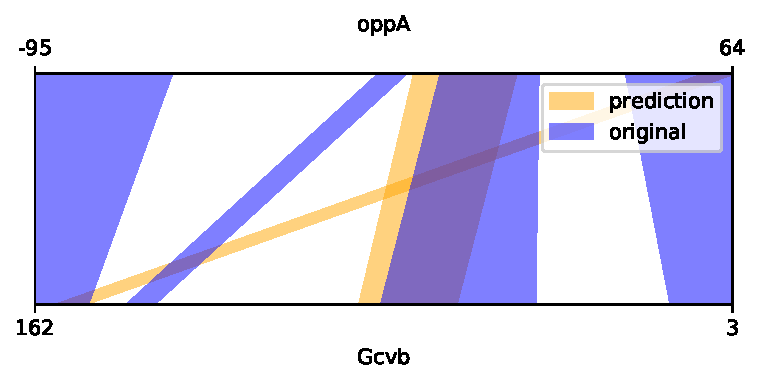
\includegraphics[width=.5\linewidth]{rricomparison6}
	\centering
	\caption{ GcvB:oppA interaction that is predicted using double-site tool. We can see that out of four original interaction blocks(blue colour), we predicted (orange colour) the interaction of two blocks. } 
	\label{fig:rricomparison6}
\end{figure}


\clearpage
	
%	\item \textbf{GcvB – cycA }
%	
%	This interaction is an example for more than two site RNA interaction. In Escherichia coli, the GcvB gene encodes a small non-translated RNA that regulates several genes involved in transport of amino acids and peptides (including sstT, oppA and dppA). Microarray analysis identified cycA as an additional regulatory target of GcvB. In addition, deletion of the GcvB gene resulted in increased sensitivity to d-cycloserine, consistent with increased expression of cycA. The total energy for both the block is -23.19.
	
	\section{DicF - ftsZ }
	
	This is an example of a crossing interaction. We note that the DicF-ftsZ complex admits an area of complementarity, which gives rise to a generalized pseudo-knot. \\   
	
	The function of DicF was predicted on the basis of the complementarity of DicF RNA with the ftsZ mRNA binding region. DicF RNA is a 53-nucleotide gene formed in certain E.coli mutants. Here, DicF RNA is an antisense regulator of ftsZ translation.\\
	
	This example is taken from the paper \citep{pervouchine2004iris}. They say that DicF RNA has substantial complementarity with ftsZ mRNA in the area surrounding the Shine Dalgarno sequence, which is compatible with the finding that DicF controls ftsZ through interaction with the ribosome binding. DicF-ftsZ complex admits the region of complementarity which leads to generalized pseudoknot (refer to Fig ~\ref{fig:dicf}). \\
	
	When we run with IntaRNA first, we observed that the Dicf (35 - 52) interacts with ftsZ (53 - 75) is the block that is predicted (52:55\&35:73) with mfe of -6.89. Then, we run them with our tool. For this example we used the parameter file and set the tIntLenMax=20 ( for restricting the overall length an interaction ).The total interaction energy for two sides of block that has been predicted by the tool is -13.86 \\
	
		\begin{figure}[h!tb]
		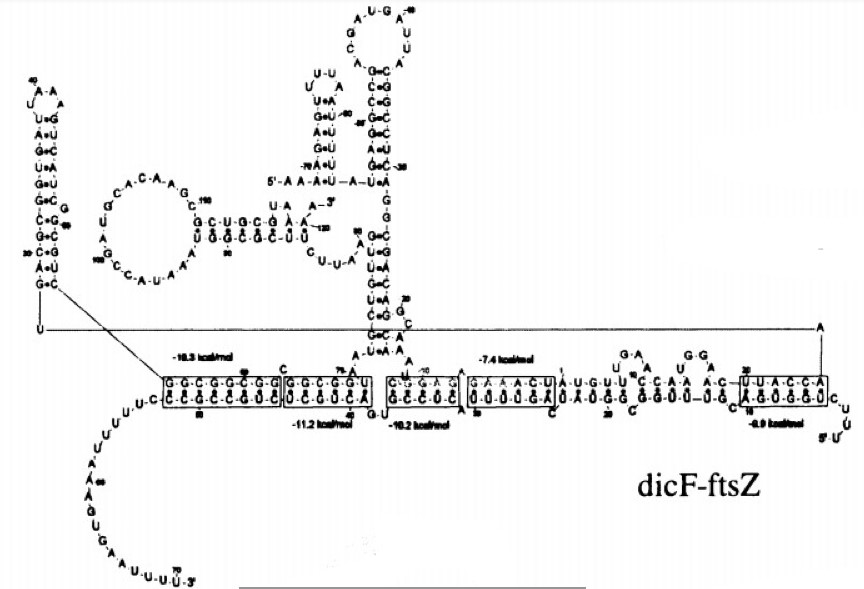
\includegraphics[width=1.0\linewidth]{dicf}
		\centering
		\caption{ Interaction of DicF - ftsZ which has a generalized pseudoknot structure that has been predicted by IRIS.  Figure is taken from the paper \citep{pervouchine2004iris}. } 
		\label{fig:dicf}
	\end{figure}

\begin{figure}[h!tb]
	\centering
	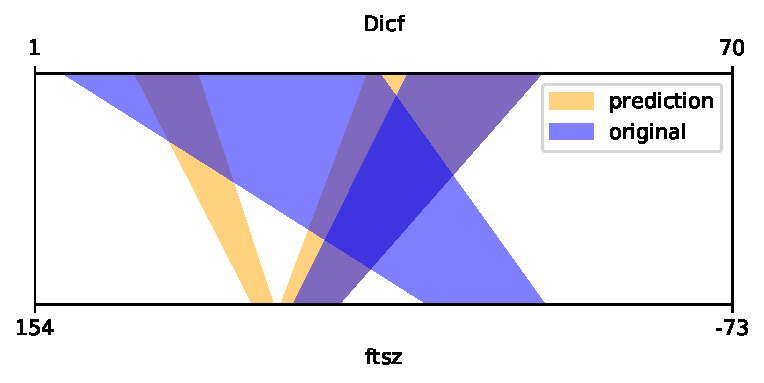
\includegraphics[width=.4\linewidth]{rricomparison3}
	\caption{DicF:ftsZ interaction that is predicted using double-site tool. We can see that the original interaction blocks(blue colour) form a crossing structure, whereas the predicted (orange colour) blocks doesn't.}
	\label{fig:rricomparison3}
\end{figure}

\clearpage
	\section{S-mRNA - EGS }
	
	 In all species ribonuclease P (RNase P) was found. External guide sequences (EGSs) are RNA molecules consisting of a sequence complementary to mRNA targeting and recruiting intracellular ribonuclease P (RNase P), a tRNA processing enzyme, for target mRNA specific degradation. EGS  RNAs  derived  from  natural  tRNA sequences can be good in blocking gene expression in  bacteria.\\
	 
	 This example is taken from the paper {\citep{zhang2013engineered}}. It is possible that an improvement in the RNase P cleavage rate could be attributed to additional tertiary interactions that theoretically stabilize the mRNA-EGS complex. Variant C386 was chosen for this analysis because the EGS RNAs derived from this version are among the most efficient EGS's. EGS S-C386 was built by connecting the EGS domain of C386 to targeting sequences complementary to the S mRNA. The EGS, S-SER, originating from the normal tRNASer series, was also built. If this is the case, the binding affinity of the EGS variant (i.e. S-C386) to the target S RNA sequence might be greater than that of the EGS (i.e. S-SER) derived from the normal tRNA sequence. We couldn't reproduce the structures from literature for any of the sequence pairs.\\
	 
	 S-C386-C and S-SER-C were derived from S-C386 and S-SER, respectively, and incorporated simple substitutions (5'-UUC-3'- > AAG) at the three closely conserved locations in the T-loop of these EGSs. Nucleotides in these three positions are highly conserved among tRNA molecules and are essential for the folding and recognition of tRNA molecules by RNase P, so mutations in these positions are involved in the EGS process. S-C386-C and S-SER-C had the same anti-sense pattern to the targetS RNA series as S-C386 and S-SER Fig: ~\ref{fig:test1}  and had identical binding affinities to S38 as S-C386 and S-SER, respectively. S-C386-Cand S-SER-C can also be used as anti-sense regulation of such EGSs.\\
	   
	 
	 Due to its very short sequence Fig: ~\ref{fig:test1}, we took the 50nt long on the left side and right side of UCUUCAUCCUGCUGCUAUGCCUCAUCUUC of S-mRNA. When we run with IntaRNA first, we observed that the mRNA (-1 - 7) interacts with EGS S-SER \& SER-C (46 - 53) ie.,-1:53\&7:46 is the block that is predicted for both mRNA:EGS S-SER and mRNA:EGS S-SER-C with mfe of -8.41. The total energy for mRNA:EGS S-C386 is -14.14, mRNA:EGS S-C386C is -13.24, mRNA:EGS S-SER and mRNA:EGS S-SER-C is -16.0.  Here, the start of the S-mRNA is complementary to the end of the S-SER, which led to the crossing pattern.  \\
	 

	 
	 \begin{figure}[h!tb]
	 	\centering
	 	\begin{subfigure}{.25\textwidth}
	 		\centering
	 		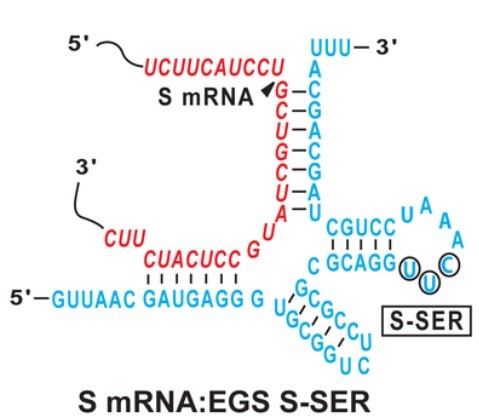
\includegraphics[width=.9\linewidth]{mrnaegs}	
	 		\label{fig:mrnaegs}
	 	\end{subfigure}%
		\begin{subfigure}{.5\textwidth}
			\centering
			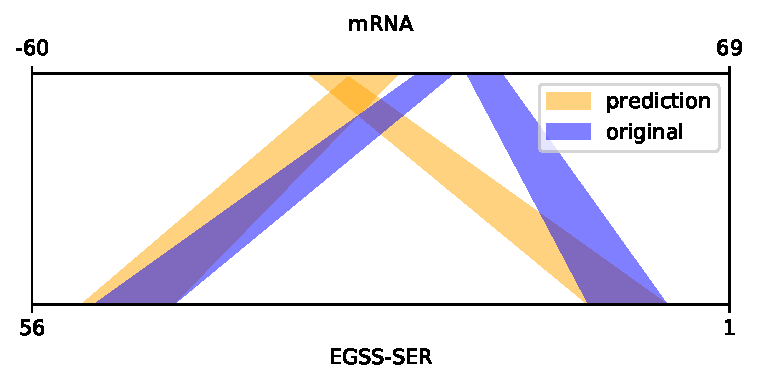
\includegraphics[width=.9\linewidth]{rricomparison7}
			\caption{mRNA:EGS S-SER}
			\label{fig:rricomparison7}
		\end{subfigure}
	 	\begin{subfigure}{.25\textwidth}
	 		\centering
	 		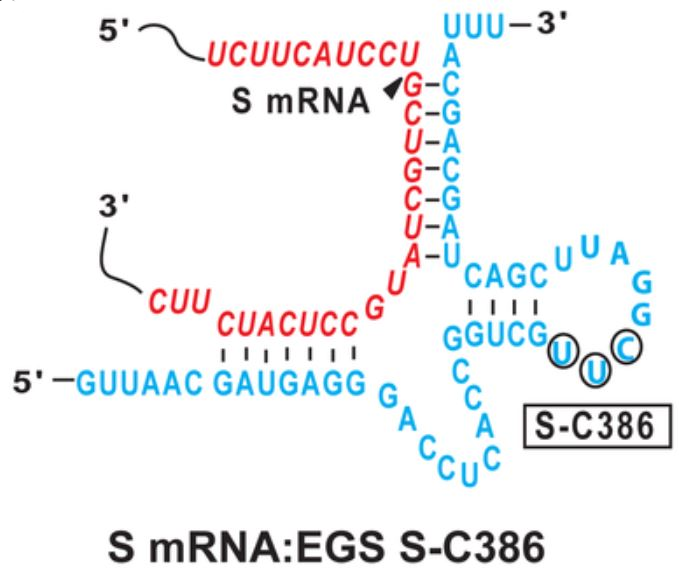
\includegraphics[width=.9\linewidth]{SC386}
	 		\label{fig:SC386}
	 	\end{subfigure}%
 	\begin{subfigure}{.5\textwidth}
 		\centering
 		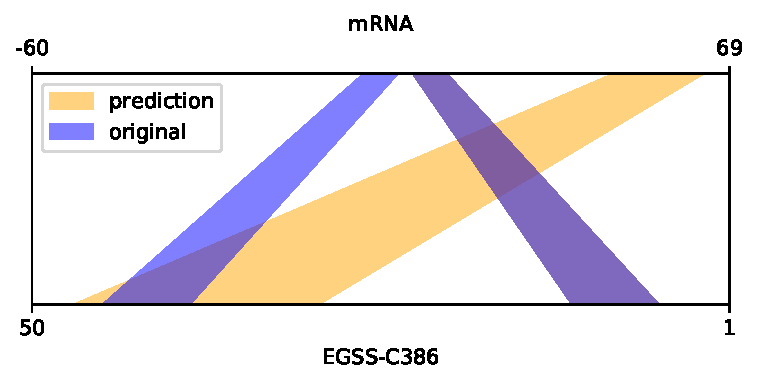
\includegraphics[width=.9\linewidth]{rricomparison4}
 		\caption{mRNA:EGS S-C386}
 		\label{fig:rricomparison4}
 	\end{subfigure}
	 	\begin{subfigure}{.25\textwidth}
	 		\centering
	 		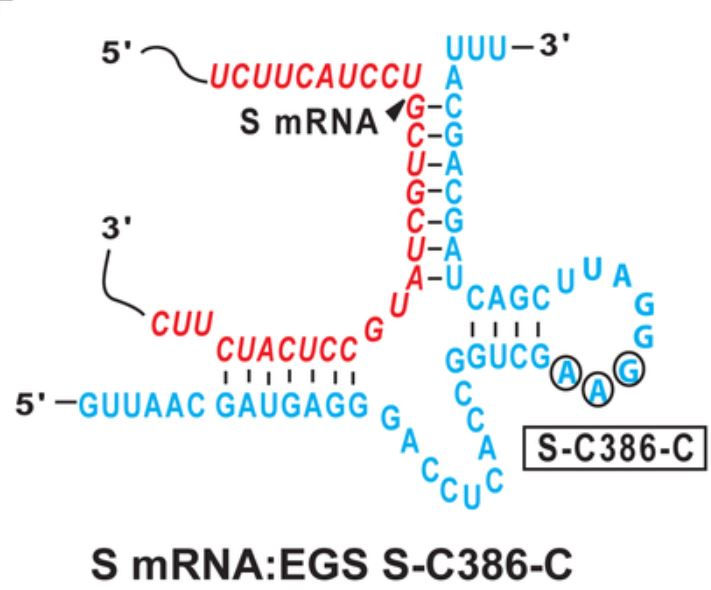
\includegraphics[width=.9\linewidth]{sc386c}
	 	
	 		\label{fig:sc386c}
	 	\end{subfigure}%
 	\begin{subfigure}{.5\textwidth}
 		\centering
 		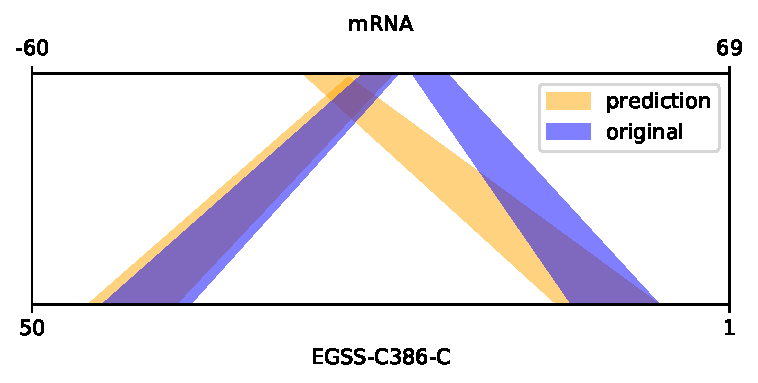
\includegraphics[width=.9\linewidth]{rricomparison5}
 		\caption{mRNA:EGS S-C386-C}
 		\label{fig:rricomparison5}
 	\end{subfigure}
	 	\begin{subfigure}{.25\textwidth}
	 		\centering
	 		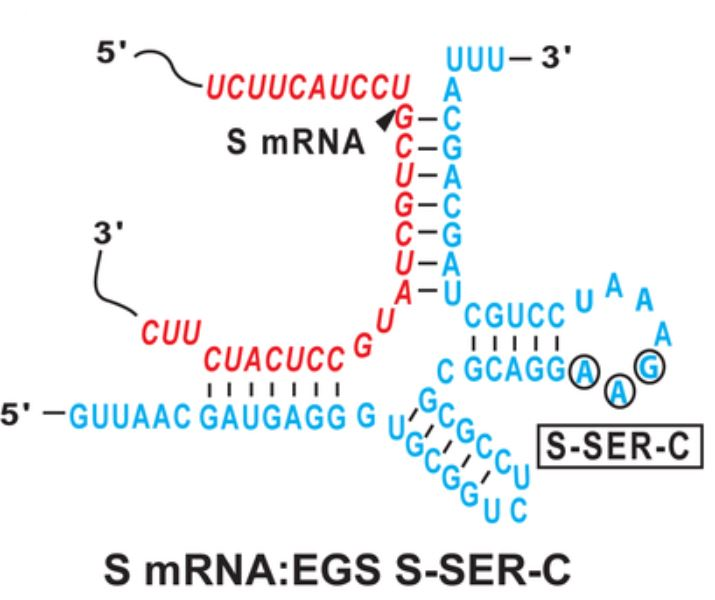
\includegraphics[width=.9\linewidth]{SERC}
	 		
	 		\label{fig:SERC}
	 	\end{subfigure}%
 	\begin{subfigure}{.5\textwidth}
 		\centering
 		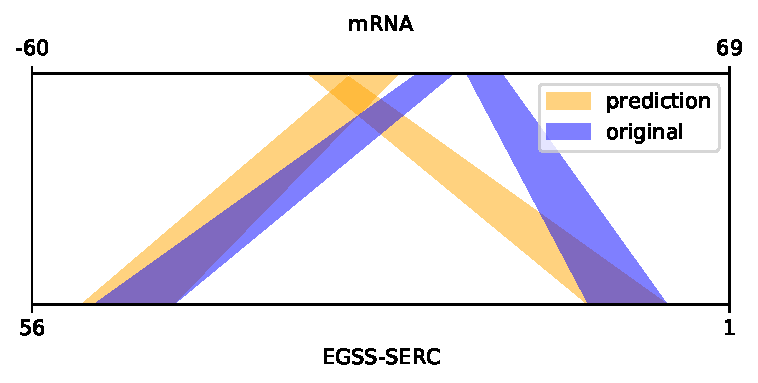
\includegraphics[width=.9\linewidth]{rricomparison8}
 		\caption{mRNA:EGS S-SERC}
 		\label{fig:rricomparison8}
 	\end{subfigure}
 	\caption{An EGS resembling the structure of a tRNA. The left side of the figure is taken from the paper \citep {zhang2013engineered}. The site of cleavage by RNase P is marked with an arrowhead, S mRNA (red color) and the EGS (blue color). The right side is the predicted structure from the tool. Original interaction blocks(blue colour) and the predicted blocks (orange colour). Just the exact sequence of the S mRNA around the targeting region is displayed (in red) and the EGS sequence is shown in blue. The RNase P cleavage site is labelled with an arrowhead. The sequences of S-SER and S-SER-C relative to T-stem and loop and the variable area of the tRNA molecule were derived from tRNASer, while those of S-C386 and S-C386-C were derived from the EGS variant C386. The index position is taken from the site of cleavage.\\ }
	 	\label{fig:test1}
	 \end{figure}
	 
%	 \begin{figure}[h!tb]
%	 	\centering
%	 \begin{subfigure}{.5\textwidth}
%	 	\centering
%	 	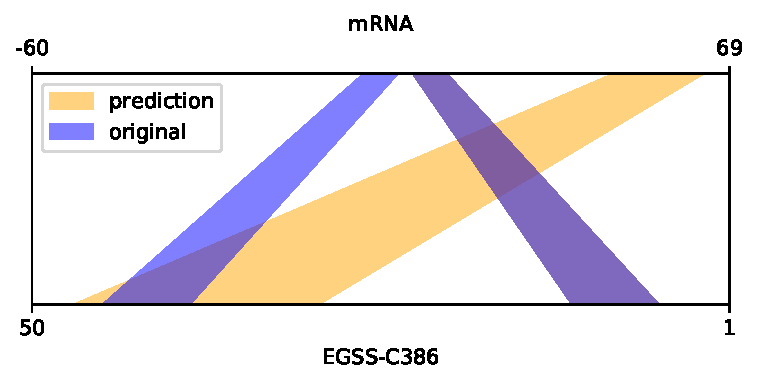
\includegraphics[width=.9\linewidth]{rricomparison4}
%	 	\caption{mRNA:EGS S-C386}
%	 	\label{fig:rricomparison4}
%	 \end{subfigure}%
%	 \begin{subfigure}{.5\textwidth}
%	 	\centering
%	 	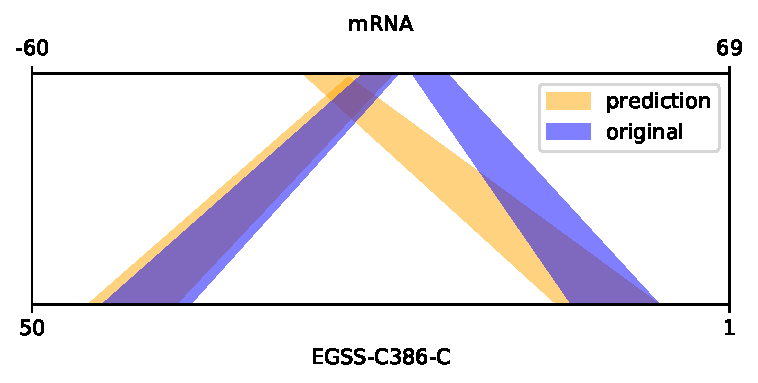
\includegraphics[width=.9\linewidth]{rricomparison5}
%	 	\caption{mRNA:EGS S-C386-C}
%	 	\label{fig:rricomparison5}
%	 \end{subfigure}
% \begin{subfigure}{.5\textwidth}
% 	\centering
% 	\includegraphics[width=.9\linewidth]{rricomparison7}
% 	\caption{mRNA:EGS S-SER}
% 	\label{fig:rricomparison7}
% \end{subfigure}%
% \begin{subfigure}{.5\textwidth}
% 	\centering
% 	\includegraphics[width=.9\linewidth]{rricomparison8}
% 	\caption{mRNA:EGS S-SERC}
% 	\label{fig:rricomparison8}
% \end{subfigure}%
% \end{figure}
\clearpage	


\section{Details of studied RRIs}

Below is the table for the comparison between the different interacting RNAs that are used for the study purpose within this thesis. The table provides us with the original interaction from the paper and the prediction's from the tool. The table also clearly tells us that $E(B1+ B2)$ the multi-site energy is almost double the single site energy $E(B1)$. 1st Index gives us with the index positions and the length determines the sequence length.\\
	
\begin{table}[H]
	

	\begin{tabular}{ |p{2cm}|p{2.8cm}|p{2.8cm}|p{1cm}|p{1cm}|p{1cm}|p{1cm}|}
	
		\hline
		query:target& original& prediction& \rotatebox[origin=c]{90} {E(B1)}  &\rotatebox[origin=c]{90}{E(B1+B2)}  &\rotatebox[origin=c]{90}{1st index}  &\rotatebox[origin=c]{90}{length} \\
		\hline
		\hline
		OxyS:fhlA&104:-15\&98:-9 30:34\&22:42
		&104:-15\&98:-9 30:24\&24:40&-4.37 &-7.99 &1:-53&109:113\\
		\hline
		Spot42:sthA&55:15\&48:22  7:NA\&5:NA & 55:15\&34:40 7:-8\&1:-2
		& -7.85 &-13.05 & 1:-75 &109:150 \\
		\hline
		oppA:GcvB &-95:163\&-64:151 -17:142\&-11:136 -3:84\&19:49 39:18\&64:1  &14:67\&-9:89 63:152\&57:158
		
		& -14.57 &-26.38 & -95:3 &159:160\\
		\hline
		%			GcvB:cycA&  &161:175\&62:277 40:91\&34:97	& -18.88 &-23.19 & &201:300 \\
		%			\hline
		DicF:ftsZ&52:55\&39:69   \hbox{36:-12\&5:25}  &52:55\&35:73 12:82\&18:76	& -6.89 &-13.86 &1:-73 &70:227 \\
		\hline
		mRNA:EGSS-SER &16:7\&10:13 7:46\&1:52
		  &-1:53\&7:46 \hbox{-9:13\&-3:7}
		 & -8.41 &-16.0 & -60:1 &129:156 \\
		\hline
		mRNA:EGSS-SER-C &16:7\&10:13 7:46\&1:52
		  &-1:53\&7:46 \hbox{-9:13\&-3:7}
		 & -8.41 &-16.0 & -60:1 &129:156 \\
		\hline
		mRNA:EGS S-C386 &1:46\&7:40 10:13\&16:7 &
		47:48\&63:31 10:13\&16:7
		  & -8.15&-14.14 & -60:1 &129:150 \\
		\hline
		mRNA:EGS S-C386-C &1:46\&7:40 10:13\&16:7
		 &-1:47\&6:41 \hbox{-10:14\&-3:7}
		  & -8.67 &-13.24 & -60:1 &129:150 \\
		\hline
	\end{tabular}
	\caption{Collections of multisite RNA interaction. The query and target are the RNAs interacting. ":" is used to differentiate between the query and target , "\&" is used for the differentiate between start and end of the blocks.  }	
		\label{table:2}
\end{table}



	
%	\chapter{Discussion and conclusion}
%	
%	Here in the chapter we will discuss about the result section briefly.
%	
%	
%	\section{OxyS – fhlA}
%	
%	 \section{Spot42 – sthA }
%	 
%
%
%	  
%	  \section{gcvB – oppA }
%	 
%	
%	 \section{DicF - ftsZ }
%	 
%	 
%	 \section{S-mRNA:EGS  }
%	 
	
		\chapter{Summary}
		
	The motivation of the thesis is to efficiently predict concurrent blocks of interaction within an accessibility-based prediction model. Here, we use a Single-site RNA-RNA interaction prediction tool (namely IntaRNA) for the prediction of Multi-site RNA-RNA interaction. Due to the time constraint, we have implemented the double-site interaction here by using an iterative scheme. In the iterative scheme we block the interaction site and fixing the conditional site while running the IntaRNA tool. Until we get the convergence, we iterate. The theoretical approach of multi-site interaction scheme has also been discussed. Future work on the multi-site interaction can be implemented based on the theoretical approach that has been discussed above ( refer to section 2.4). \\
	
	 The proof and implementation of double-site interaction model has been developed within this thesis. The theory proof of energy of an respective Multi-site RNA-RNA interaction can be computed from the two energies was developed and shown in the section 2.3. Then the idea has been implemented by using python based on IntaRNA calls. The double-site interaction study says that interaction energy for two blocks B1 and B2 together often double the minimum free energy. The detailed study of such examples are given in a table ~\ref{table:2} for the easy comparison. \\
	 
	  We collected some sample Multi-site RNA-RNA interaction examples from literature. The examples with the crossing interaction (pseudoknot), with two intermolecular helices, kissing interaction,etc., are used for the study purpose. We used the python polygon plots for plotting the blocks that are predicted. Then, we compared the outcome with extracted data from literatures. Each example shows its own structure, but most of them were very well close to the original one's that is taken from the literature. The brief explanation of the each study has been given in the chapter 3. \\ 
	  
	  
	
	
%	RNA interaction prediction is still an expanding field. The future work that can extended beyond this thesis, one possible idea would be the multi-site prediction. For multi-site interaction, we need to fix two conditional site and iterate it until it converges.  \\
	
	
	\bibliographystyle{plainnat}
	\bibliography{ref}
	
\begin{appendices}

	\chapter{RNA Sequences}
	
	\begin{table}[H]
		\tiny
	\begin{tabular}{ |l | l| }
		\hline
		RNA& Sequence\\
		\hline\hline	
		OxyS&
		GAAACGGAGCGGCACCTCTTTTAACCCTTGAAGTCACTGCCCGTTTCGAGAGTTTCTCAACTCGAATAACTAAAGC
		\\
		&CAACGTGAACTTTTGCGGATCTCCAGGATCCGC \\
		\hline
		fhlA&
		AGTTAGTCAATGACCTTTTGCACCGCTTTGCGGTGCTTTCCTGGAAGAACAAAATGTCATATACACCGATGAGTGA
		\\&TCTCGGACAACAAGGGTTGTTCGACATCACTCGGACA\\
		\hline
		Spot42&
		GUAGGGUACAGAGGUAAGAUGUUCUAUCUUUCAGACCUUUUACUUCACGUAAUCGGAUUUGGCUGAAUAUUUUAGC
		\\&CGCCCCAGUCAGUAAUGACUGGGGCGUUUUUUA\\
			\hline
		sthA&
		GGGATCAATTGGCTTACCCGCGATAAAATGTTACCATTCTGTTGCTTTTATGTATAAGAACAGGTAAGCCCTACCA
		\\&TGCCACATTCCTACGATTACGATGCCATAGTAATAGGTTCCGGCCCCGGCGGCGAAGGCGCTGCAATGGGCCTG\\
			\hline	
		gcvB &
		TTCCTGAGCCGGAACGAAAAGTTTTATCGGAATGCGTGTTCTGATGGGCTTTTGGCTTACGGTTGTGATGTTGTGT
		\\&
		TGTTGTGTTTGCAATTGGTCTGCGATTCAGACCACGGTAGCGAGACTACCCTTTTTCACTTCCTGTACATTTACCC
		\\&TGTCTGTC\\
		\hline
		oppA& GACAGCAGAAAGUCUCCGAGCCUGUGCAGGGUCCCAAUCCGGGAUUACACAUGCUGGUUAAUACCAGUAAUUAUAA
		\\&
		UGAGGGAGUCCAAAAAACAAUGACCAACAUCACCAAGAGAAGUUUAGUAGCAGCUGGCGUUCUGGCUGCGCUAAUG
		\\&GCAGGGA\\
		\hline
		DicF& TTTCTGGTGACGTTTGGCGGTATCAGTTTTACTCCGTGACTGCTCTGCCGCCCTTTTTAAAGTGAATTTT\\
		\hline
		ftsZ& AAAAGAGTTTTAATTTTTATGAGGCCGACGATGATTACGGCCTCAGGCGACAGGCACAAATCGGAGAGAAACTATG
		\\&
		TTTGAACCAATGGAACTTACCAATGACGCGGTGATTAAAGTCATCGGCGTCGGCGGCGGCGGCGGTAATGCTGTTG
		\\&
		AACACATGGTGCGCGAGCGCATTGAAGGTGTTGAATTCTTCGCGGTAAATACCGATGCACAAGCGCTGCGTAAAA\\	
			\hline
		EGS& AACTTGTCCTGGTTATCGCTGGATGTGTCTGCGGCGTTTTATCATCTTCCTCTTCATCCTGCTGCTATGCCTCATC
		\\&TTCTTGTTGGTTCTTCTGGACTATCAAGGTATGTTGCCCGTTTGTCCTCTAAT\\
			\hline
			S-SER& GTTAACGATGAGGGTGCGGTCTCCGCGCGCAGGTTCAAATCCTGCTAGCAGCATTT\\
			\hline
			S-SER-C&GTTAACGATGAGGGTGCGGTCTCCGCGCGCAGGAAGAAATCCTGCTAGCAGCATTT\\
			\hline
			S-C386&GTTAACGATGAGGGACCTCACCGGTCGTTCGGATTCGACTAGCAGCATTT\\
			\hline
			S-C386C& GTTAACGATGAGGGACCTCACCGGTCGAAGGGATTCGACTAGCAGCATTT\\
			\hline
	\end{tabular}
\caption{Table of RNAs with their corresponding sequence as used in this thesis.}
\end{table}

	
\end{appendices}
	
\end{document}